% Mini project report, LNMIIT. Layout follows the department's B.Tech. project report sample.
% Build: ml/.venv/bin/python docs/mini-project-report/build.py   (fills generated/values.tex, draws the figures, compiles)
\documentclass[12pt,a4paper,oneside]{report}

\usepackage[a4paper,left=33mm,right=33mm,top=30mm,bottom=28mm,headheight=15pt,headsep=14mm]{geometry}
\usepackage{fontspec}
\setmainfont{texgyretermes}[Extension=.otf,UprightFont=*-regular,BoldFont=*-bold,ItalicFont=*-italic,BoldItalicFont=*-bolditalic]
\usepackage{unicode-math}
\setmathfont{texgyretermes-math.otf}
\newfontfamily\rupeefont{Georgia.ttf}[Path=/System/Library/Fonts/Supplemental/,Scale=0.95]
\newcommand{\rupee}{{\rupeefont ₹}}
\newfontfamily\devafont{DevanagariMT.ttc}[Path=/System/Library/Fonts/Supplemental/]
\newfontfamily\codefont{DejaVuSansMono}[Extension=.ttf,UprightFont=*,BoldFont=*-Bold,Scale=0.82]

\usepackage{setspace}
\setstretch{1.42}
\usepackage[hidelinks]{hyperref}
\usepackage{graphicx,booktabs,tabularx,multirow,array,float,enumitem,xcolor}
\usepackage[labelfont=sc,labelsep=colon,font=small,skip=6pt]{caption}
\usepackage{titlesec}
\usepackage{fancyhdr}
\usepackage[titles]{tocloft}
\usepackage{listings}
\usepackage{tikz}
\usetikzlibrary{positioning,arrows.meta,fit,backgrounds,calc,shapes.geometric}

\graphicspath{{generated/fig/}{figures/}}
\input{generated/values.tex}

% ---------- headings: "Chapter N" over a large title, as in the sample
\titleformat{\chapter}[display]{\bfseries}{\fontsize{22}{26}\selectfont\chaptertitlename\ \thechapter}{28pt}{\fontsize{30}{34}\selectfont}
\titlespacing*{\chapter}{0pt}{60pt}{40pt}
\titleformat{\section}{\fontsize{15}{18}\selectfont\bfseries}{\thesection}{1em}{}
\titleformat{\subsection}{\fontsize{13}{16}\selectfont\bfseries}{\thesubsection}{1em}{}
\titleformat{\paragraph}[runin]{\bfseries}{}{}{}[.]
\titlespacing*{\section}{0pt}{22pt}{10pt}
\titlespacing*{\subsection}{0pt}{16pt}{8pt}
\setcounter{secnumdepth}{2}
\setcounter{tocdepth}{2}

% ---------- running header: "chapter: 01" ... page, with a rule
\newcommand{\twodigit}[1]{\ifnum#1<10 0\fi\number#1}
\pagestyle{fancy}
\fancyhf{}
\renewcommand{\headrulewidth}{0.5pt}
\fancyhead[L]{\itshape\markname}
\fancyhead[R]{\thepage}
\newcommand{\markname}{}
\fancypagestyle{plain}{\fancyhf{}\renewcommand{\headrulewidth}{0pt}\fancyfoot[C]{\thepage}}
\renewcommand{\chaptermark}[1]{\renewcommand{\markname}{chapter: \twodigit{\value{chapter}}}}

% ---------- lists, captions, tables
\setlist{itemsep=2pt,topsep=4pt}
\renewcommand{\cftchapfont}{\bfseries}
\renewcommand{\cftchappagefont}{\bfseries}
\renewcommand{\cftfigfont}{\figurename~}
\renewcommand{\cfttabfont}{\tablename~}
\setlength{\cftfignumwidth}{2.6em}
\setlength{\cfttabnumwidth}{2.6em}
\captionsetup[table]{position=above}
\newcolumntype{L}[1]{>{\raggedright\arraybackslash}p{#1}}
\newcolumntype{Y}{>{\raggedright\arraybackslash}X}
\newcolumntype{R}[1]{>{\raggedleft\arraybackslash}p{#1}}
\renewcommand{\arraystretch}{1.25}

% ---------- code listings (appendix)
\lstset{basicstyle=\codefont\footnotesize,breaklines=true,columns=fullflexible,keepspaces=true,frame=lines,framesep=4pt,
  numbers=left,numberstyle=\tiny\color{gray},xleftmargin=1.5em,showstringspaces=false,
  keywordstyle=\bfseries,commentstyle=\itshape\color{gray},upquote=true,literate={−}{{-}}1 {×}{{x}}1 {≥}{{>=}}1 {≤}{{<=}}1 {→}{{->}}1 {÷}{{/}}1 {₹}{{Rs}}2 {—}{{--}}1 {–}{{-}}1 {…}{{...}}1 {·}{{.}}1}

% ---------- TikZ styles shared by the diagrams
\tikzset{
  box/.style={draw=black!55,rounded corners=2pt,align=center,font=\small,inner sep=4pt,minimum height=8mm,fill=#1},
  box/.default=black!4,
  arr/.style={-{Stealth[length=2mm]},draw=black!65,thick},
  grp/.style={draw=#1,dashed,rounded corners=4pt,inner sep=6pt},
  note/.style={font=\scriptsize\itshape,text=black!60,align=left},
}
\colorlet{cA}{blue!8}\colorlet{cB}{red!9}\colorlet{cC}{green!10}\colorlet{cD}{orange!12}

% "pending" marker for results that the LoRA experiment will fill in
\newcommand{\pending}{\textit{pending}}

\begin{document}

% ================================================================== title page
\begin{titlepage}
\setstretch{1.15}
\centering
\vspace*{6mm}
{\fontsize{20}{25}\selectfont\bfseries Garment-to-Model Virtual Try-On\\for Small Online Sellers\par}
\vspace{6mm}
{\large\itshape A Serving System for FASHN VTON 1.5, a LoRA Adaptation Pipeline\\and a Catalogue-Driven Content Engine\par}
\vspace{8mm}
{\large Mini Project Report, B.Tech.\ Fifth Semester\par}
\vspace{10mm}
{\large Project report submitted in partial fulfillment\\of the requirements for the degree of\par}
\vspace{5mm}
{\large\itshape Bachelor of Technology\\in\\Electronics and Communication Engineering /\\Computer Science and Engineering\par}
\vspace{6mm}
{\large by\par}
\vspace{5mm}
{\large Amrendra Vikram Singh - Roll No. 24UEC092\\Avirat Kaushik - Roll No. 24UCS235\par}
\vspace{8mm}
{\large Under the Guidance of\\Dr. Nishant Gupta\par}
\vspace{8mm}

\includegraphics[width=36mm]{figures/lnmiit-logo.png}\par
\vspace{8mm}
{\large The LNM Institute of Information Technology, Jaipur\par}
\vspace{4mm}
{\large November 2026\par}
\end{titlepage}

\thispagestyle{empty}
\vspace*{\fill}
\begin{center}\bfseries ©The LNM Institute of Information Technology, Jaipur - 2026.\\All rights reserved.\end{center}
\vspace{20mm}
\clearpage

\pagenumbering{roman}
\setcounter{page}{3}
\renewcommand{\markname}{}

% ================================================================== certificate
\thispagestyle{empty}
\vspace*{22mm}
\begin{center}
{\Large The LNM Institute of Information Technology\\Jaipur, India\par}
\vspace{22mm}
{\Large\bfseries CERTIFICATE\par}
\end{center}
\vspace{10mm}
\noindent This is to certify that the project entitled ``Garment-to-Model Virtual Try-On for Small Online Sellers'', submitted by Amrendra Vikram Singh (Roll No.~24UEC092) and Avirat Kaushik (Roll No.~24UCS235) in partial fulfillment of the requirement of degree in Bachelor of Technology (B.Tech.), is a bonafide record of work carried out by them at The LNM Institute of Information Technology, Jaipur (Rajasthan), India, as the fifth-semester mini project during the academic session 2026-2027 under my supervision and guidance, and the same has not been submitted elsewhere for award of any other degree. In my opinion, this report is of the standard required for the award of the degree of Bachelor of Technology (B.Tech.).

\vspace{24mm}
\noindent\rule{62mm}{0.4pt}\\
Guide: Dr. Nishant Gupta

\vspace{12mm}
\noindent Date: \rule{38mm}{0.4pt}
\clearpage

% ================================================================== acknowledgments
\chapter*{Acknowledgments}
\thispagestyle{plain}
We thank our guide, Dr.\ Nishant Gupta, for taking on a project that sits between computer vision, systems engineering and small-business marketing, and for the questions that shaped how we report it: what exactly is ours, what was measured, and what is still only a plan.

We thank the Department of Electronics and Communication Engineering and the Department of Computer Science and Engineering at LNMIIT for the opportunity to work on an open-ended problem in the fifth semester.

The try-on model at the centre of this work, FASHN VTON 1.5, was released openly by FASHN AI under the Apache-2.0 licence, and its hosted demonstration runs on Hugging Face's shared GPUs. Without both, a project with no budget could not have produced a single image.

Parts of the code and of this write-up were drafted with the help of an AI coding assistant. We reviewed, ran and tested what it produced, and every number in this report comes from a file the project's own scripts generate; Appendix~A lists the command behind each one.

\vspace{18mm}
\begin{flushright}Amrendra Vikram Singh\\Avirat Kaushik\end{flushright}

% ================================================================== abstract
\chapter*{Abstract}
\thispagestyle{plain}
\renewcommand{\markname}{Abstract}
Small clothing sellers in India usually have one flat photograph of each garment, while buyers decide faster when they see it worn. This project builds a free system that puts a garment photograph onto a model, turns the result into an Instagram post and advises the seller on price, wording and timing.

The try-on model is FASHN VTON 1.5, an open 972-million-parameter diffusion transformer that combines a person photograph and a garment photograph through joint attention, directly in pixel space. We did not train it. We built the system around it: a single orchestration function that checks a content-addressed cache and a running-job table before it queues for the shared GPU, a photo-cleaning stage, live progress streaming, and a ledger that learns the free GPU quota. Over \vNRuns{} real generations a new photo took a median of \vMedTotal{}~s, of which \vMedGpu{}~s was GPU time; a repeat request was answered from the cache in \vCacheMs{}~ms.

The model was released without training code. We reconstructed its training objective from the sampler and confirmed it on the released weights (a loss \vLossRatio{} times lower than under the opposite convention), then built a LoRA fine-tuning pipeline: \vTrainParamsM{}M trainable parameters (\vLoraPct{}\%) on \vLoraLayers{} layers, a \vAdapterMb{}~MB adapter, and a training state of \vLoraStateGb{}~GB against \vFullStateGb{}~GB for full fine-tuning. A data pipeline turns a retail catalogue into training pairs with pose and image guardrails\ifPairs{} (\vPairsN{} pairs from \vPairsProducts{} products, with no product family in both training and validation)\fi. \ifLora Trained for \vLcSteps{} steps at \vLcScale{} resolution on the laptop and compared with the base model on \vLcN{} held-out garments, the adapter changed the denoising error from \vLcDlBase{} to \vLcDlLora{} (\vLcDlRel{}\%, 95\% CI of the difference \vLcDlCi{}; \vLcDlVerdict{}); on the \vLcGen{} garments generated as images, PSNR went from \vLcPsnrBase{} to \vLcPsnrLora{}~dB (\vLcPsnrVerdict{}) and garment-pixel error from \vLcGlBase{} to \vLcGlLora{} (\vLcGlVerdict{}).\else The comparison of the adapted and the base model on held-out garments is specified and automated but has not been run yet; its numbers are marked as pending throughout and no improvement in try-on quality is claimed.\fi

The content side calls free language models through one validated function and keeps all arithmetic and dates in code. \ifMarket From \vMkTotalClean{} cleaned listings (T-shirts and tops from Amazon.in, sarees and kurta sets from Myntra) it derives price bands, demand shares and title keywords; median discounts of \vMkTeeDisc{}--\vMkKurtaDisc{}\% turn out to be at most weakly related to demand. Pricing, title, hashtag, positioning and location engines use these statistics; for a kurta-set seller in Jaipur they recommend \rupee\vExBandLo{}--\rupee\vExBandHi{} among \vExComparables{} comparable listings.\fi

\vspace{6pt}\noindent\textbf{Keywords:} virtual try-on, diffusion transformer, rectified flow, LoRA, parameter-efficient fine-tuning, pose estimation, caching, e-commerce analytics, small businesses.

% ================================================================== lists
\clearpage
\renewcommand{\markname}{CONTENTS}
\tableofcontents
\clearpage
\renewcommand{\markname}{LIST OF FIGURES}
\listoffigures
\clearpage
\renewcommand{\markname}{LIST OF TABLES}
\listoftables
\clearpage
\renewcommand{\markname}{List of Abbreviations}
\chapter*{List of Abbreviations}
\addcontentsline{toc}{chapter}{List of Abbreviations}
\thispagestyle{plain}
\begin{tabular}{@{}p{30mm}p{110mm}@{}}
API & Application programming interface\\
CFG & Classifier-free guidance\\
CI & Confidence interval\\
DiT & Diffusion transformer\\
DWPose & Whole-body pose estimator used by FASHN VTON\\
EXIF & Exchangeable image file format (photo metadata)\\
GEO & Geographic targeting (city and regional calendar)\\
GPU & Graphics processing unit\\
HHI & Herfindahl--Hirschman index of concentration\\
IQR & Interquartile range\\
LLM & Large language model\\
LoRA & Low-rank adaptation\\
MLP & Multi-layer perceptron\\
MMDiT & Multimodal diffusion transformer\\
MRP & Maximum retail price\\
NDJSON & Newline-delimited JSON\\
PSNR & Peak signal-to-noise ratio\\
RoPE & Rotary position embedding\\
SEO & Search engine optimisation\\
SSIM & Structural similarity index\\
VAE & Variational autoencoder\\
VTON & Virtual try-on\\
ZeroGPU & Hugging Face's shared, on-demand GPU service\\
\end{tabular}

\clearpage
\pagenumbering{arabic}
\chapter{Introduction}

\section{The Area of Work}

A large share of India's clothing trade now happens through small sellers on Instagram, WhatsApp and marketplaces such as Meesho and Amazon. A typical seller works from home or a small shop, buys or makes a few dozen pieces at a time, and photographs each one on a bed, a hanger or a mannequin. Large brands show the same kind of garment on a professional model, shot in a studio and edited by a designer. A model shoot costs thousands of rupees a day, which a seller with forty kurtis to list cannot pay.

The difference matters because buyers decide faster when they can see how a garment falls on a body. A flat photograph shows the colour and the print but not the length, the fit or the drape. Virtual try-on, the computer-vision task of generating a photograph of a given person wearing a given garment, addresses exactly this gap. Over the last two years diffusion models have made the generated images good enough to use, and in early 2026 an open model, FASHN VTON 1.5, was released that accepts the flat photographs these sellers actually have.

A try-on photograph is only the first step. The seller still has to write a caption, choose a price, decide what to post and when, and pick hashtags that buyers search for. This project sits where generative image models, systems engineering for free compute, and the practical marketing questions of a small seller meet.

\section{Problem Addressed}

Three problems come together in this project.

\begin{enumerate}
\item \textbf{Generating the photograph for free.} The model needs a GPU with about 8~GB of memory. A seller has none, and neither did we: on our laptop one photograph took \vGenMinutes{} minutes. The only free option is a shared GPU service with a small, partly unpublished daily quota, which has to be protected from waste.
\item \textbf{Adapting the model to Indian garments.} The model was trained mostly on Western clothing and was released without any training code, so nobody outside the company can teach it a kurti, a saree or a lehenga.
\item \textbf{Turning the photograph into a sale.} A caption, a price and a posting plan written by a language model can contain invented prices, wrong arithmetic and made-up statistics, which harm a seller far more than a plain template would.
\end{enumerate}

\noindent The question we set out to answer is therefore:

\begin{quote}\itshape
Can a small seller's single flat garment photograph be turned, at no cost, into an on-model photograph and a trustworthy post and pricing plan, and can the try-on model be adapted to the seller's own garments in a way that can be measured?
\end{quote}

\paragraph{Scope of this report} The try-on network is FASHN AI's, and we did not train it from scratch. Our work is the system around it, the reconstruction of its training method, the adaptation pipeline with its guardrails and evaluation, and the content engines. \ifLora The adapter reported here was trained on our 8~GB laptop at half resolution for about an hour; it shows a measured improvement on held-out garments under a strict claim rule, but a full-resolution run on a CUDA GPU, and Indian garments, remain future work.\else The adapted model has not yet been trained, because that needs a CUDA GPU; every place where its results belong is marked \pending{}, and no improvement from fine-tuning is claimed in this version.\fi

\section{How the Work Was Organised}

The project ran over the fifth semester in three tracks that share one codebase (Figure~\ref{fig:roadmap}).

\begin{figure}[!htbp]
\centering
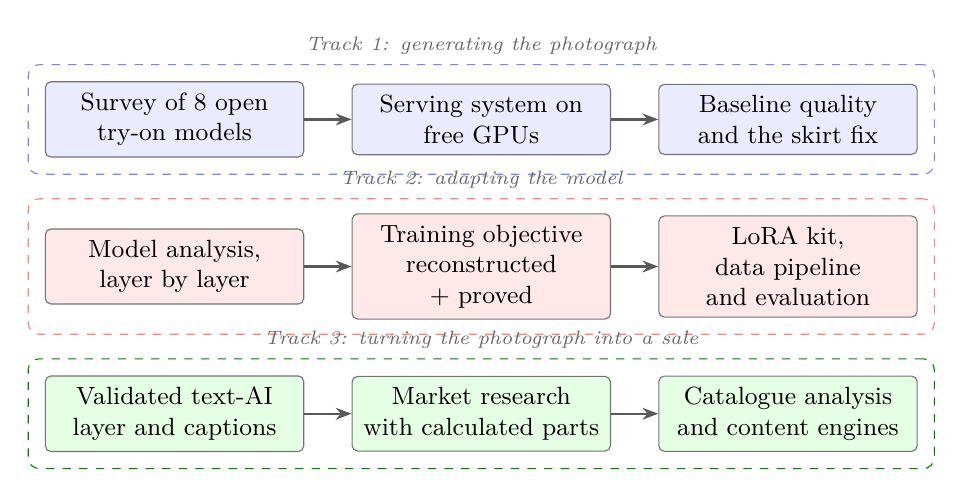
\begin{tikzpicture}[node distance=5mm and 6mm]
\node[box=cA,text width=30mm] (a1) {Survey of 8 open\\try-on models};
\node[box=cA,text width=30mm,right=of a1] (a2) {Serving system on\\free GPUs};
\node[box=cA,text width=30mm,right=of a2] (a3) {Baseline quality\\and the skirt fix};
\node[box=cB,text width=30mm,below=9mm of a1] (b1) {Model analysis,\\layer by layer};
\node[box=cB,text width=30mm,right=of b1] (b2) {Training objective\\reconstructed + proved};
\node[box=cB,text width=30mm,right=of b2] (b3) {LoRA kit, data pipeline\\and evaluation};
\node[box=cC,text width=30mm,below=9mm of b1] (c1) {Validated text-AI\\layer and captions};
\node[box=cC,text width=30mm,right=of c1] (c2) {Market research\\with calculated parts};
\node[box=cC,text width=30mm,right=of c2] (c3) {Catalogue analysis\\and content engines};
\draw[arr] (a1)--(a2); \draw[arr] (a2)--(a3); \draw[arr] (b1)--(b2); \draw[arr] (b2)--(b3); \draw[arr] (c1)--(c2); \draw[arr] (c2)--(c3);
\begin{scope}[on background layer]
\node[grp=blue!50,fit=(a1)(a3),label={[note]above:Track 1: generating the photograph}] {};
\node[grp=red!50,fit=(b1)(b3),label={[note]above:Track 2: adapting the model}] {};
\node[grp=green!50!black,fit=(c1)(c3),label={[note]above:Track 3: turning the photograph into a sale}] {};
\end{scope}
\end{tikzpicture}
\caption{The three tracks of the project and the order in which each was built.}
\label{fig:roadmap}
\end{figure}

\section{How the Work Evolved}

The project went through three stages: a first working studio, a measured and corrected version, and the present version with the adaptation pipeline and the content engines. Table~\ref{tab:evolution} summarises what changed at each stage and why.

\begin{table}[!htbp]
\centering
\caption{Evolution of the project.}
\label{tab:evolution}
\small
\begin{tabularx}{\linewidth}{@{}L{25mm}YYY@{}}
\toprule
\textbf{Aspect} & \textbf{First version (early Oct.)} & \textbf{After the baseline (late Oct.)} & \textbf{This report (Nov.)}\\
\midrule
Try-on & One call to the hosted model & One entry point with cache, job sharing and a GPU lock & Same, with a measured cache path\\
Model photos & Any preset & Presets carry what they wear; bottoms go to a model in separates & Same\\
Quality & Not measured & 4 try-ons scored on a 30-point rubric & Plus PSNR, SSIM and garment error in the LoRA evaluation\\
Training & None possible & Objective reconstructed, LoRA kit with 12 tests & Checked on the real weights; 100-step run; catalogue-to-pairs pipeline\\
Text & Captions from one model & Validated provider chain, price check, templates & Plus catalogue-driven pricing, title, hashtag and location engines\\
Market data & None & Seller's answers, calendar in code, AI advice & Plus demand and price statistics from \ifMarket\vMkTeeClean{} + \vMkTopClean{}\else catalogue\fi{} listings\\
\bottomrule
\end{tabularx}
\end{table}

\section{Overall System Architecture}

Figure~\ref{fig:arch} shows the complete system. The browser sends the garment photograph, the choice of model and the settings. The server cleans the photographs, decides whether any GPU work is needed at all, and sends the job to the try-on model on Hugging Face's free GPU service. The result is saved and streamed back while it is being made. The same server calls free language models for captions and research, always through one validating function, and the catalogue analysis supplies the numbers the content engines use. The adaptation pipeline on the right runs offline and produces an adapter file that a future engine would load.

\begin{figure}[!htbp]
\centering
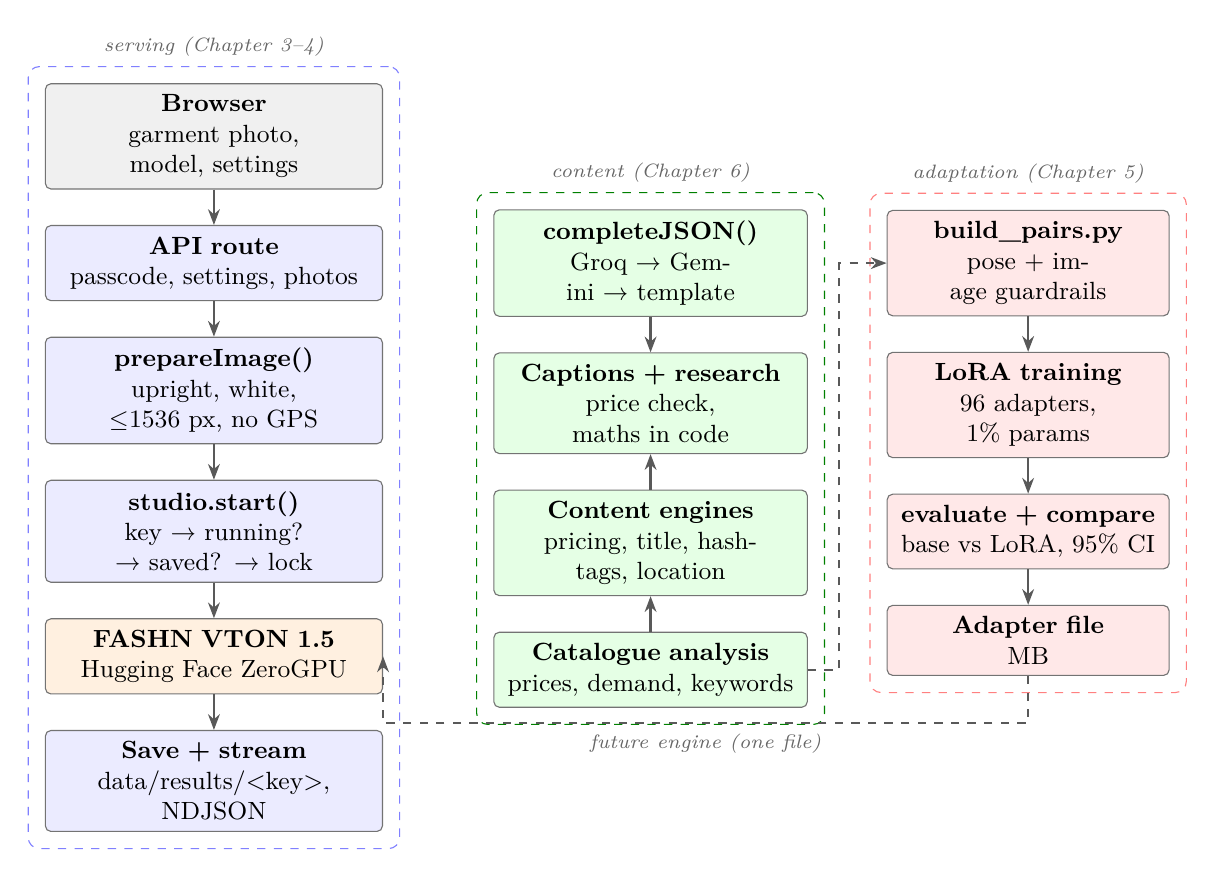
\begin{tikzpicture}[node distance=4.5mm]
\node[box=black!6,text width=40mm] (br) {\textbf{Browser}\\garment photo, model, settings};
\node[box=cA,text width=40mm,below=of br] (rt) {\textbf{API route}\\passcode, settings, photos};
\node[box=cA,text width=40mm,below=of rt] (pi) {\textbf{prepareImage()}\\upright, white, $\le$1536 px, no GPS};
\node[box=cA,text width=40mm,below=of pi] (st) {\textbf{studio.start()}\\key → running? → saved? → lock};
\node[box=cD,text width=40mm,below=of st] (fa) {\textbf{FASHN VTON 1.5}\\Hugging Face ZeroGPU};
\node[box=cA,text width=40mm,below=of fa] (sv) {\textbf{Save + stream}\\data/results/<key>, NDJSON};
\draw[arr] (br)--(rt); \draw[arr] (rt)--(pi); \draw[arr] (pi)--(st); \draw[arr] (st)--(fa); \draw[arr] (fa)--(sv);
\node[box=cC,text width=37mm,right=14mm of rt] (cj) {\textbf{completeJSON()}\\Groq → Gemini → template};
\node[box=cC,text width=37mm,below=of cj] (cp) {\textbf{Captions + research}\\price check, maths in code};
\node[box=cC,text width=37mm,below=of cp] (en) {\textbf{Content engines}\\pricing, title, hashtags, location};
\node[box=cC,text width=37mm,below=of en] (mk) {\textbf{Catalogue analysis}\\prices, demand, keywords};
\draw[arr] (cj)--(cp); \draw[arr] (mk)--(en); \draw[arr] (en)--(cp);
\node[box=cB,text width=33mm,right=10mm of cj] (bp) {\textbf{build\_pairs.py}\\pose + image guardrails};
\node[box=cB,text width=33mm,below=of bp] (tr) {\textbf{LoRA training}\\96 adapters, 1\% params};
\node[box=cB,text width=33mm,below=of tr] (ev) {\textbf{evaluate + compare}\\base vs LoRA, 95\% CI};
\node[box=cB,text width=33mm,below=of ev] (ad) {\textbf{Adapter file}\\\vAdapterMb{} MB};
\draw[arr] (bp)--(tr); \draw[arr] (tr)--(ev); \draw[arr] (ev)--(ad);
\draw[arr,dashed] (ad.south) |- ++(0,-6mm) -| node[note,pos=0.25,below]{future engine (one file)} (fa.east);
\draw[arr,dashed] (mk.east) -- ++(4mm,0) |- (bp.west);
\begin{scope}[on background layer]
\node[grp=blue!50,fit=(br)(sv),label={[note]above:serving (Chapter 3--4)}] {};
\node[grp=green!50!black,fit=(cj)(mk),label={[note]above:content (Chapter 6)}] {};
\node[grp=red!50,fit=(bp)(ad),label={[note]above:adaptation (Chapter 5)}] {};
\end{scope}
\end{tikzpicture}
\caption{End-to-end architecture. Blue: serving the try-on; green: text and market intelligence; red: offline adaptation of the model. Dashed arrows are links that are designed but not yet live.}
\label{fig:arch}
\end{figure}

\section{Objectives}

The specific objectives of the project were:

\begin{enumerate}
\item Serve an open try-on model to sellers at zero cost, without wasting the small free GPU quota, and with honest progress and error messages.
\item Understand the try-on network layer by layer, from its released source code, well enough to explain where the garment's detail enters the person's image.
\item Make the model trainable: recover the training objective it was trained with and prove it against the released weights.
\item Build a parameter-efficient adaptation pipeline, from raw retail catalogue photographs to training pairs, with guardrails on pose and photo quality, and an evaluation protocol that decides when an improvement may be claimed.
\item Give the seller trustworthy text: captions, a pricing band, a product title, hashtags and a posting calendar, with every number computed in code.
\item Measure every part and report what was not done.
\end{enumerate}

\section{Contributions}

The network and its weights are not our contribution. Our contributions are:

\begin{itemize}
\item \textbf{A serving system for a free, rate-limited GPU.} One entry point checks a content-addressed cache and a running-job table before it waits for the GPU, cancels abandoned queue places, and learns the provider's unpublished daily run limit from its refusal messages.
\item \textbf{A verified training objective for a model released without one.} The rectified-flow objective was derived from the sampler and confirmed on the real weights; our inference code reproduces FASHN's output exactly (mean difference \vEquivDiff{} of 255).
\item \textbf{A LoRA adaptation pipeline.} \vLoraLayers{} adapters (\vLoraPct{}\% of the parameters), a garment-weighted loss, new garment categories, a catalogue-to-pairs pipeline with pose guardrails, and a base-versus-adapter evaluation with confidence intervals.
\item \textbf{Guardrails and evaluations for the model's output.} Five checks on every generated photograph in the application (two reject, three warn), calibrated on our real generations, and model-level evaluations of pose drift and garment colour error with pass rates for the base and the adapted model.
\item \textbf{A finding about the licence.} The only non-commercial component, the human parser, has no effect on the output in the mode the application uses (difference \vParserDiff{} of 255), so it can be removed.
\item \textbf{Catalogue-driven content engines} that keep language models away from numbers, with a demand analysis of real listings.
\end{itemize}

\section{Organisation of the Report}

Chapter~2 reviews the literature behind each part. Chapter~3 describes the serving system and its pipeline. Chapter~4 explains the try-on model layer by layer. Chapter~5 presents the proposed adaptation work: the reconstructed objective, the LoRA adapters, the data pipeline with its guardrails, the evaluation protocol and the compute cost. Chapter~6 covers the text-AI layer, the market analysis and the content engines. Chapter~7 presents all results, and Chapter~8 concludes. Appendix~A lists the command behind every number, and Appendix~B the most important code.

\chapter{Literature Review}

\section{Introduction}

The project draws on four bodies of work: image-based virtual try-on, the diffusion and flow models that now generate the images, parameter-efficient fine-tuning, and the use of marketplace signals such as ratings as evidence of demand. This chapter reviews each in turn and ends with the gap the project addresses.

\section{Base Model of the Project}

FASHN VTON 1.5~\cite{fashn} is the model this project serves and adapts. It was released by FASHN AI in 2026 as weights and inference code under the Apache-2.0 licence, with a model card but without a paper or training code. It has 972 million parameters, generates directly in pixel space at 864$\times$576, accepts a garment photographed flat or worn by another person, and needs no mask of the region to replace. Its architecture adapts the multimodal diffusion transformer of FLUX.1~\cite{flux}: the garment image takes the place of the text prompt. The model card reports training on about 18 million image pairs and a generation time of about 5~s on an NVIDIA H100. Chapter~4 describes the network in detail.

We chose it after comparing eight open models and several paid services. Table~\ref{tab:choice} gives the deciding properties for the most relevant alternatives.

\begin{table}[!htbp]
\centering
\caption{Open try-on models considered (from their public repositories, September 2026).}
\label{tab:choice}
\small
\begin{tabularx}{\linewidth}{@{}L{24mm}L{22mm}L{22mm}YL{18mm}@{}}
\toprule
\textbf{Model} & \textbf{Flat-lay input} & \textbf{Mask needed} & \textbf{Licence of weights} & \textbf{Space}\\
\midrule
FASHN VTON 1.5~\cite{fashn} & yes & no & Apache-2.0 & official, free\\
IDM-VTON~\cite{idmvton} & yes & yes & CC BY-NC-SA 4.0 (non-commercial) & yes\\
CatVTON~\cite{catvton} & yes & yes & CC BY-NC-SA 4.0 (non-commercial) & error\\
OOTDiffusion~\cite{ootd} & yes & yes & CC BY-NC-SA 4.0 (non-commercial) & yes\\
Leffa~\cite{leffa} & yes & yes & MIT (preprocessing has other terms) & yes\\
\bottomrule
\end{tabularx}
\end{table}

\noindent Only FASHN VTON 1.5 combines the three properties a seller needs: it takes the photograph the seller already has, it asks nothing more of the seller, and its licence does not forbid later commercial use.

\section{Image-Based Virtual Try-On}

VITON~\cite{viton} defined the task with a two-stage design: the clothing region of the person is removed, the garment image is warped to the body with a thin-plate spline, and a refinement network blends the two. CP-VTON~\cite{cpvton} learned the warp instead of fixing its form, and VITON-HD~\cite{vitonhd} raised the resolution to 1024$\times$768 and released the dataset that became the standard benchmark. Dress Code~\cite{dresscode} added lower-body garments and dresses as separate categories, which is the category split FASHN VTON also uses.

Warping-based methods keep the garment's texture well wherever the warp is correct. They fail when an arm crosses the body, when the pose differs strongly from the garment photograph, or when the garment changes shape on the body, because a flat image cannot be bent into every three-dimensional configuration.

\section{Diffusion Models for Try-On}

Denoising diffusion models~\cite{ddpm} generate an image by learning to reverse a gradual noising process. Latent diffusion~\cite{ldm} made them practical at high resolution by working in the compressed space of an autoencoder (VAE), at the cost of an 8$\times$ spatial compression that blurs small details such as printed text.

TryOnDiffusion~\cite{tryondiff} replaced the warp with two communicating U-Nets, one for the person and one for the garment. OOTDiffusion~\cite{ootd} and IDM-VTON~\cite{idmvton} feed features from a separate garment encoder into the denoising network through attention. CatVTON~\cite{catvton} showed that simply placing the garment and the person side by side in the input is enough. Leffa~\cite{leffa} adds a loss that guides attention towards the corresponding garment region. All of these work in a latent space and all need a mask that fixes, in advance, the region the garment may occupy.

\section{Transformers and Rectified Flow}

The transformer~\cite{transformer} processes a sequence of tokens with attention, in which every token builds its output from a weighted combination of all the others. The Diffusion Transformer~\cite{dit} replaced the U-Net with a transformer over image patches. Rotary position embeddings~\cite{rope} encode where each patch lies by rotating its query and key vectors, so that attention depends on relative position.

Rectified flow~\cite{rectflow} and flow matching~\cite{flowmatch} recast generation as following a straight path from noise to data. A network learns the velocity along that path, and sampling integrates it with a few Euler steps. Stable Diffusion~3~\cite{sd3} combined these ideas in the multimodal diffusion transformer (MMDiT), in which image tokens and text tokens keep separate weights but attend to each other jointly, and introduced a logit-normal sampling of training time steps. FLUX.1~\cite{flux} added single-stream blocks in which both sequences share weights. FASHN VTON 1.5 inherits all of these choices.

\section{Classifier-Free Guidance}

Classifier-free guidance~\cite{cfg} trains a single network both with and without its conditions, by dropping the conditions for a fraction of training examples. At sampling time the two predictions are combined, $v = v_\varnothing + s\,(v_c - v_\varnothing)$, and a scale $s > 1$ pushes the result towards following the condition more closely. This doubles the cost of every sampling step. It also places a requirement on any fine-tuning: the conditions must still be dropped during training, or guidance stops working.

\section{Parameter-Efficient Fine-Tuning}

Fine-tuning all parameters of a large model on a small dataset is expensive and tends to overwrite what the model learned before. Adapter layers~\cite{adapters} insert small trainable modules into a frozen network. LoRA~\cite{lora} instead learns a low-rank update to an existing weight matrix,
\begin{equation}
W' = W + \frac{\alpha}{r} BA, \qquad B \in \mathbb{R}^{d_\text{out}\times r},\ A \in \mathbb{R}^{r\times d_\text{in}},\ r \ll \min(d_\text{in}, d_\text{out}),
\end{equation}
with $B$ initialised to zero so that training starts from exactly the pretrained model. The update can be merged into $W$ after training, so it adds no cost at inference, or kept separate and switched on and off. QLoRA~\cite{qlora} showed that the frozen weights can even be kept in reduced precision while the adapters train. Gradient checkpointing~\cite{checkpoint} trades recomputation for activation memory, and AdamW~\cite{adamw} is the usual optimiser for both full and low-rank fine-tuning.

\section{Pose Estimation}

Try-on models need to know where the body is. OpenPose~\cite{openpose} introduced the 18-keypoint body skeleton that is still used as the drawing format. FASHN VTON uses a YOLOX~\cite{yolox} person detector followed by DWPose~\cite{dwpose}, a distilled whole-body estimator that predicts 133 keypoints (body, feet, face and hands) with a confidence for each. Our data pipeline (Chapter~5) reuses these two networks as guardrails on training photographs. A SegFormer~\cite{segformer} human parser, which labels each pixel with a body part or garment class, is also part of FASHN's pipeline and is the only component with a non-commercial licence.

\section{How Try-On Results Are Evaluated}

Papers on paired data report PSNR and SSIM~\cite{ssim}, which compare a generated image with the real photograph pixel by pixel and structurally, and LPIPS~\cite{lpips}, a learned perceptual distance. On unpaired data they report FID~\cite{fid}, which compares the statistics of thousands of generated and real images. None of these measures checks directly whether a logo or a price tag is reproduced correctly, which is why we also use a garment-only pixel error and a rubric. When two models are compared on the same samples, a paired test such as the Wilcoxon signed-rank test~\cite{wilcoxon} and bootstrap confidence intervals~\cite{bootstrap} say whether a difference is larger than chance. Splitting training and test data by individual photograph instead of by product leaks information and inflates results~\cite{leakage}; we split by product family.

\section{Marketplace Signals as Evidence of Demand}

Sales figures of marketplace listings are not public. The number of ratings or reviews a listing has accumulated is visible, and work in marketing has used review volume as a measure of sales and has shown that reviews influence sales~\cite{wom}. We use the number of ratings as a demand signal, state the assumption explicitly, and give unit estimates only as a range. Rank correlation~\cite{spearman} measures association between price, discount and demand without assuming a linear relation.

\section{General Image Models and Language Models}

General image generators, including those built into chat assistants, can place a garment on a person from a text instruction. They are trained to produce a plausible picture, not to preserve a specific product's print and logo, they cannot be studied or retrained by a user, and they charge per image. For text, free tiers of language models (Groq~\cite{groq}, Gemini~\cite{gemini}) answer in an OpenAI-compatible format, but their output can contain invented prices and arithmetic errors, which is why every call in this project is validated and every number is computed in code.

\section{What the Literature Does Not Provide}

The literature gives strong try-on models, but none that is at the same time open for commercial use, mask-free, flat-lay capable and trainable by its users: FASHN VTON 1.5 meets the first three and not the last. It gives a general method for cheap adaptation (LoRA) but no recipe for this model and no public paired dataset of Indian garments. It gives metrics for image similarity but no guidance on serving such a model on a free, rate-limited GPU, and no tools that connect a generated photograph to the seller's pricing and wording. This project addresses these gaps.

\chapter{The Serving System and Its Pipeline}

\section{Overview}

The application, Haat Studio, is a Next.js~16 web application written in TypeScript (about 7{,}700 lines). Its job in the try-on path is to take a seller's request, decide whether any GPU work is needed at all, get the work done on a free shared GPU, and return the result while being honest about every stage. The design follows one rule: every try-on in the application, whether started from a web page, a script or an evaluation, goes through a single function, \texttt{studio().start()}. Because there is only one entry point, no route can skip its protections.

Figure~\ref{fig:journey} shows the life of one request.

\begin{figure}[!htbp]
\centering
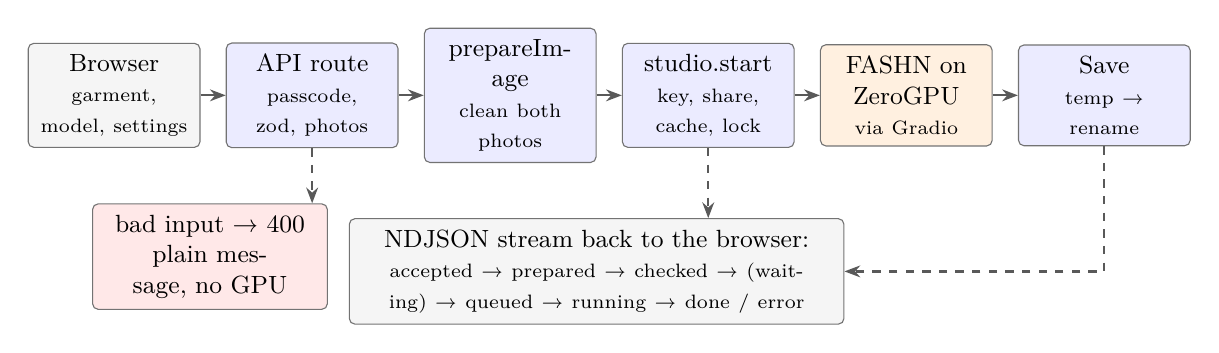
\begin{tikzpicture}[node distance=3.2mm]
\node[box,text width=19mm] (b) {Browser\\\scriptsize garment, model, settings};
\node[box=cA,text width=19mm,right=of b] (r) {API route\\\scriptsize passcode, zod, photos};
\node[box=cA,text width=19mm,right=of r] (p) {prepareImage\\\scriptsize clean both photos};
\node[box=cA,text width=19mm,right=of p] (s) {studio.start\\\scriptsize key, share, cache, lock};
\node[box=cD,text width=19mm,right=of s] (f) {FASHN on\\ZeroGPU\\\scriptsize via Gradio};
\node[box=cA,text width=19mm,right=of f] (v) {Save\\\scriptsize temp → rename};
\draw[arr] (b)--(r); \draw[arr] (r)--(p); \draw[arr] (p)--(s); \draw[arr] (s)--(f); \draw[arr] (f)--(v);
\node[box=black!4,text width=60mm,below=7mm of p.south east,anchor=north] (st) {NDJSON stream back to the browser:\\\scriptsize accepted → prepared → checked → (waiting) → queued → running → done / error};
\draw[arr,dashed] (s.south) -- (s.south|-st.north);
\draw[arr,dashed] (v.south) |- (st.east);
\node[box=cB,text width=27mm,below=7mm of r.south,anchor=north east,xshift=2mm] (e) {bad input → 400\\plain message, no GPU};
\draw[arr,dashed] (r.south) -- (r.south|-e.north);
\end{tikzpicture}
\caption{The journey of one try-on request. Input problems are answered at once with a plain error; only valid requests start the stream.}
\label{fig:journey}
\end{figure}

\section{The API Route}

The route \texttt{POST /api/tryon} receives a multipart form: the garment photograph, either a preset model identifier or an uploaded photograph of a person, and four settings. It checks them in order of cost:

\begin{enumerate}
\item \textbf{Passcode.} On a public deployment every route that creates something requires a passcode, compared in constant time (\texttt{timingSafeEqual}) so that response time does not reveal how many characters were right. On a laptop no passcode is set and the check passes.
\item \textbf{Settings.} A zod schema validates the category (tops, bottoms, one-pieces), the photo type (flat-lay or worn), the quality (fast, balanced or best, meaning 20, 30 or 50 sampling steps) and the seed.
\item \textbf{Photographs.} A garment photograph must be present, and either a preset or an uploaded person.
\end{enumerate}

\noindent Problems with the request come back as an ordinary error before any streaming starts. The browser can therefore always tell ``fix your photo'' apart from ``the engine failed''.

\section{Cleaning the Photographs}

Before any GPU time is spent, \texttt{prepareImage()} brings both photographs into a known state (Table~\ref{tab:prep}). Each step exists because of a problem we met.

\begin{table}[!htbp]
\centering
\caption{What \texttt{prepareImage()} does to every photograph, and why.}
\label{tab:prep}
\small
\begin{tabularx}{\linewidth}{@{}L{50mm}Y@{}}
\toprule
\textbf{Step} & \textbf{Reason}\\
\midrule
Reject files over 15~MB, HEIC, and formats other than JPEG, PNG and WebP & HEIC cannot be decoded by the pipeline; the message names the iPhone setting to change\\
Apply the EXIF orientation & Phone photographs are often stored sideways with a ``rotate'' flag; the model would receive a sideways image\\
Flatten transparency onto white & The model converts transparency to black, so a cut-out product would float in a black void\\
Limit the longest side to 1{,}536~px & The model works at about 576~px wide; larger files only cost upload time\\
Remove metadata & Phone photographs carry the GPS location of the seller's home\\
Reject a short side under 256~px & Too small to produce a usable result\\
\bottomrule
\end{tabularx}
\end{table}

A photograph that is already a clean JPEG (upright, opaque, without metadata, not oversized) is passed through unchanged, byte for byte. Re-encoding it would change its bytes, which would change its cache key (Section~\ref{sec:cache}) and turn a free repeat request into a paid one. The function also returns a record of what it changed, which the progress panel shows, so the application never claims work it did not do. In our \vNRuns{} real generations, \vNPrepUntouched{} of the \vNPrepPhotos{} photographs passed through untouched.

\section{One Entry Point: \texttt{studio().start()}}
\label{sec:studio}

Figure~\ref{fig:studio} shows the decisions inside the entry point. They are ordered from the cheapest to the most expensive: memory, then disk, then the GPU.

\begin{figure}[!htbp]
\centering
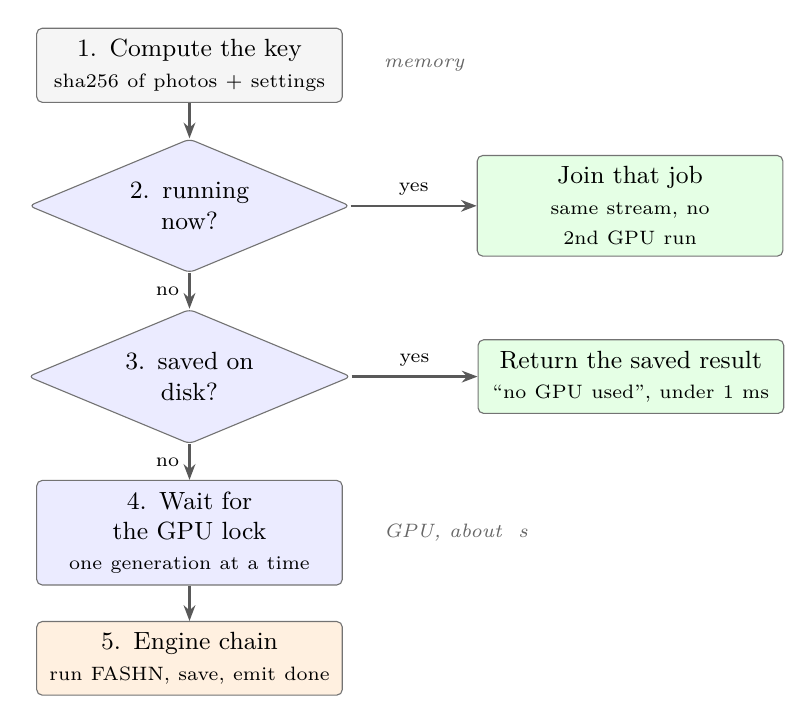
\begin{tikzpicture}[node distance=4.5mm]
\node[box,text width=36mm] (k) {1. Compute the key\\\scriptsize sha256 of photos + settings};
\node[box=cA,shape=diamond,aspect=2.4,inner sep=1pt,text width=24mm,below=of k] (r) {2. running\\now?};
\node[box=cA,shape=diamond,aspect=2.4,inner sep=1pt,text width=24mm,below=of r] (c) {3. saved on\\disk?};
\node[box=cA,text width=36mm,below=of c] (l) {4. Wait for the GPU lock\\\scriptsize one generation at a time};
\node[box=cD,text width=36mm,below=of l] (e) {5. Engine chain\\\scriptsize run FASHN, save, emit done};
\node[box=cC,text width=36mm,right=16mm of r] (j) {Join that job\\\scriptsize same stream, no 2nd GPU run};
\node[box=cC,text width=36mm,right=16mm of c] (h) {Return the saved result\\\scriptsize ``no GPU used'', under 1 ms};
\draw[arr] (k)--(r); \draw[arr] (r)--node[left,font=\scriptsize]{no}(c); \draw[arr] (c)--node[left,font=\scriptsize]{no}(l); \draw[arr] (l)--(e);
\draw[arr] (r)--node[above,font=\scriptsize]{yes}(j); \draw[arr] (c)--node[above,font=\scriptsize]{yes}(h);
\node[note,right=4mm of k] {memory};
\node[note,right=4mm of l] {GPU, about \vMedTotal{} s};
\end{tikzpicture}
\caption{Decisions inside \texttt{studio().start()}, cheapest first.}
\label{fig:studio}
\end{figure}

\paragraph{Joining a running job} The entry point keeps a table of jobs that are running, keyed by the request key. A double click, or a second browser tab with the same photographs and settings, finds the job already in the table and subscribes to it. The GPU runs once and both pages receive the same events.

\paragraph{The GPU lock} Different requests wait for each other: a promise chain lets only one generation hold the GPU at a time, and a waiting request sends a \texttt{waiting} event so its page can say so. Two jobs racing into the free GPU would only waste the shared quota.

\paragraph{A job outlives its page} The job runs independently of the HTTP connection that started it. If the seller closes the tab, the job continues and the result is still saved, so GPU time already spent is never wasted.

\section{Engines and Errors}

An engine is anything that can perform a try-on. Every engine implements one small interface: an identifier, whether it is configured, and a \texttt{run()} function that reports progress events and returns image bytes. Adding an engine, such as a paid API or our own GPU serving the adapted model, means adding one file and one line to a registry. Today there are two: \texttt{fashn-space}, which sends the job to FASHN's official Hugging Face Space through the Gradio client~\cite{gradio}, and \texttt{echo}, a labelled test engine that returns the model photograph unchanged and is kept in a separate cache namespace so that a test image can never be served as a real one.

The free Space returns no error codes, only messages, so \texttt{classify()} reads the wording and assigns one of five kinds (Table~\ref{tab:errors}). It even reads the refill time from messages such as ``Try again in 0:13:21''.

\begin{table}[!htbp]
\centering
\caption{Error kinds and what the engine chain does with each.}
\label{tab:errors}
\small
\begin{tabularx}{\linewidth}{@{}L{24mm}YL{40mm}@{}}
\toprule
\textbf{Kind} & \textbf{Example} & \textbf{Action}\\
\midrule
input & unreadable photograph & stop: every engine would reject it\\
quota & ``exceeded your ZeroGPU runs limit'' & record the refusal, try the next engine\\
timeout & no result within 240~s & cancel our queue place, try the next\\
unavailable & ``no GPU was available'', Space asleep & try the next engine\\
unknown & anything else & try the next engine\\
\bottomrule
\end{tabularx}
\end{table}

Each generation gets 240~seconds. On a timeout the engine cancels its place in the Space's queue; otherwise a request the seller has given up on would still be run later and spend quota. Every attempt is recorded, not only the last, and \texttt{explain()} turns the list into one sentence the seller can act on, for example: \emph{``Today's free GPU quota is used up. It refills in about 14 min.''}

\section{The Cache Key and Storage}
\label{sec:cache}

The key of a request is a hash of its content:
\begin{equation}
\text{key} = \operatorname{sha256}\big(\operatorname{sha256}(g) \,|\, \operatorname{sha256}(p) \,|\, \text{category} \,|\, \text{photoType} \,|\, \text{quality} \,|\, \text{seed}\big)_{[0:32]},
\end{equation}
where $g$ and $p$ are the bytes of the cleaned garment and person photographs. Because it depends on contents and not on file names, the same photograph uploaded twice under different names is the same request. ``Another variation'' changes only the seed, which gives a new key and therefore a new image.

Results are stored in \texttt{data/results/<key>/} as \texttt{result.png}, the two input photographs and \texttt{meta.json}. They are written to a temporary folder, with \texttt{meta.json} written last, and the folder is then renamed into place. A rename is a single step, so a crash can never leave a half-written result that looks complete; the presence of \texttt{meta.json} is what marks a result as finished. Failed generations are not stored. Keys arriving in URLs are checked against \verb|^[0-9a-f]{32}$| before they touch the file system, which prevents path traversal.

\paragraph{Instagram sizes} The post (4:5, 1080$\times$1350), square (1:1) and story (9:16, 1080$\times$1920) versions are made on request with the \texttt{sharp} library and are not stored. The photograph is never cropped, because a crop could cut off the hem or the feet, which are part of the product. It is scaled to fit inside the frame,
\begin{equation}
s = \min\!\left(\frac{W}{w}, \frac{H}{h}\right),
\end{equation}
and the margins are filled with a blurred ($\sigma = 40$), slightly darkened copy of the same photograph. This darkening is the only colour change anywhere in the system; the garment's own colours are never altered.

\section{Live Progress and Reconnecting}

The response is an NDJSON stream: one JSON event per line, each stamped with the server's time. The events are \texttt{accepted}, \texttt{prepared}, \texttt{checked} (with whether the cache was hit), \texttt{waiting}, \texttt{queued} (with the position in the Space's queue), \texttt{running}, and finally \texttt{done} or \texttt{error}. The progress panel is computed from these events only; it never advances on a timer, so it shows real stages and real durations instead of an invented progress bar.

Each job keeps every event it has emitted. When a page reconnects with \texttt{/studio?r=<key>}, the route \texttt{GET /api/tryon/[key]} replays all events of a running job and then continues live; for a finished job it returns the saved result; otherwise it answers 404 and the studio offers to try again.

\section{Output Guardrails on Every Photograph}
\label{sec:guardrails}

A try-on model can fail silently: it can return a blank frame, return the model photograph unchanged, produce an image of the wrong shape, leave the old outfit showing, or change the person's face. Before a result is saved, \texttt{checkQuality()} (in \texttt{quality.ts}) runs five checks on small thumbnails (Table~\ref{tab:guardchecks}). Two are certain failures: the result is rejected exactly like an engine error, the next engine is tried, and the seller is told why. Three are heuristics: the result is kept, and the seller sees a note to check it before posting. Test engines are exempt because they return the model photograph on purpose.

\begin{table}[!htbp]
\centering
\caption{The output guardrails.}
\label{tab:guardchecks}
\small
\begin{tabularx}{\linewidth}{@{}L{18mm}YL{26mm}L{14mm}@{}}
\toprule
\textbf{Check} & \textbf{Measure} & \textbf{Limit} & \textbf{Effect}\\
\midrule
blank & mean per-channel standard deviation of the result & below 6 & fail\\
changed & mean absolute difference to the model photograph (0--255) & below 3 & fail\\
size & relative difference of the aspect ratio to the model photograph & above 0.08 & warn\\
colour & CIE76 $\Delta E$ of the result's garment area to the garment, minus $\Delta E$ to the old outfit in the same area & above 0, and $\Delta E$ to the garment above 15 & warn\\
person & mean absolute difference in the head region (0--255) & above 45 & warn\\
\bottomrule
\end{tabularx}
\end{table}

The colour check is relative on purpose. A first version compared the garment's colour with a fixed box on the torso, and on our real results it warned on a correct navy crop top (the box reached the dress below it) while missing the actual failure. The relative version asks a sharper question: does the garment area now look more like the new garment, or still like what the model wore before? \ifAppGuard Table~\ref{tab:guardaudit} shows it on all \vAgN{} real generations (median \vAgMs{}~ms per photograph): it warns on both photographs of the skirt on a model in a dress, the failure that scored 11/30 in Section~7.3, and on one uploaded photograph where the garment was a phone screenshot, and on none of the others; no result fails.

\begin{table}[!htbp]
\centering
\caption{Output guardrails on the project's real generations ($\triangle$ = warning).}
\label{tab:guardaudit}
\footnotesize
\setlength{\tabcolsep}{3.5pt}
\input{generated/app_guardrails.tex}
\end{table}
\fi

\section{The Seller's Interface}
\label{sec:ui}

The application is organised like a professional campaign tool: a sidebar with the four tools (Try-on Studio, Post Maker, Market Research, Library) and Help, a top bar with the free-GPU meter, the language switch (English or Hindi) and a Help button, and content that uses the full width of the screen. Every tool follows the same guided flow, ending in a \emph{Review} step that summarises every choice with an Edit link, the expected time and the quota it will use, before anything is created (Figure~\ref{fig:uireview}). A ``?'' button next to every control and section explains what it does. The product step offers 38 sample garments with category tabs and search; the model step filters presets by gender, by what the model wears and by suitability for the chosen garment; a Library page lists every saved photograph, sortable and filterable. The result screen leads with the quality checks of Section~\ref{sec:guardrails} (Figure~\ref{fig:uiresult}). The interface uses Calibri (or its metric-compatible open equivalent, Carlito), meets the accessibility rules of the project (44~px controls, no text below 11~px, keyboard-operable help), and is covered by \vTestsApp{} automated tests.

\begin{figure}[!htbp]
\centering
\includegraphics[width=\linewidth]{ui-review.png}
\caption{The Review step of the try-on studio: every choice, its cost and an Edit link, before anything is created.}
\label{fig:uireview}
\end{figure}

\begin{figure}[!htbp]
\centering
\includegraphics[width=\linewidth]{ui-result.png}
\caption{The result screen: before/after slider, the quality checks (here a correct warning on the skirt placed on a model in a dress), and the next step to a post.}
\label{fig:uiresult}
\end{figure}

\section{The Free GPU Quota}

Hugging Face gives a free account about five minutes of ZeroGPU time a day~\cite{zerogpu} and, in addition, a limit on the number of runs whose value is not published. Neither balance can be queried. Every call must have the Space's declared duration (60~s by default) available before it starts, although a photograph uses only part of it. The application therefore keeps its own ledger of GPU time and computes what is left:
\begin{align}
t_\text{left} &= 300\,\text{s} - \sum_{\text{runs in the current 24-hour window}} t_i, \\
n_\text{time} &= \begin{cases} \left\lfloor \dfrac{t_\text{left} - 60}{\tilde{t}} \right\rfloor + 1 & t_\text{left} \ge 60\,\text{s} \\ 0 & \text{otherwise}\end{cases}, \qquad
n_\text{left} = \min\big(n_\text{time},\; R - n_\text{used}\big),
\end{align}
where $\tilde{t}$ is the median duration of the last ten runs (currently \vPerPhoto{}~s) and $R$ is the run limit. The window starts at the first GPU use, not at midnight. When the Space refuses a call, its message is parsed: a time refusal (``60s requested vs.\ 12s left'') replaces our estimate, and a run-limit refusal teaches $R$. On 26 October the Space refused our ninth photograph after \vUsedAtRefusal{}~s of GPU time, with ``runs limit''; since then $R = \vRunsLimit{}$. Cache hits and test engines are never counted, because they use no GPU.

\section{Security and Configuration}

There is no login. Anyone with a link could spend the free quota, so every route that creates something (try-on, caption, research, featuring) calls \texttt{requirePasscode} first, while routes that only read stay open. API keys for the GPU and the language models live in one \texttt{.env} file on the server and are never sent to the browser. The configuration is parsed and validated with zod on every call, not once at start-up, so a new key takes effect without restarting the server. Photographs are stripped of metadata, and no buyer's personal data is collected anywhere.

\section{Testing}

The application has \vTestsApp{} automated tests that run in about a second without any network access: they cover the orchestration (job sharing, the lock, the error chain), the photograph cleaning, the cache key, storage, the quota arithmetic, the text-AI chain and the caption and research logic. Language models and the GPU are replaced by fake providers passed in as arguments, so tests never spend quota. Two further commands check the outside world without spending quota: \texttt{engine:check} verifies the token, the Space's status and its API contract, and \texttt{llm:check} reports which configured language models still answer.

\chapter{The Try-On Model, Layer by Layer}

This chapter describes FASHN VTON 1.5~\cite{fashn} as it appears in its released source code (the \texttt{fashn-vton} 1.5.0 package). The network and its weights are FASHN AI's work. Understanding it in this detail was a precondition for everything in Chapter~5: an adapter can only be placed well, and a training objective only reconstructed, once it is clear where the garment's detail enters the person's image.

\section{Pre-processing}

Both photographs are resized, keeping their aspect ratio, and padded to 864$\times$576 pixels. The person's body pose is detected with YOLOX~\cite{yolox} and DWPose~\cite{dwpose} and drawn as a skeleton on a black image, each limb in its own grey level, so that left and right limbs can be told apart. A garment photographed flat receives a blank pose image; a garment worn by someone else receives that person's pose.

The pipeline offers two modes. In \emph{masked} mode a SegFormer human parser~\cite{segformer} labels the clothing region of the person, which is greyed out, and the model fills it. In \emph{segmentation-free} mode, which the hosted Space uses by default and which our application uses, the model sees the whole person and decides itself what to replace. Masked mode cannot make a garment longer than the one it replaces; segmentation-free mode can, but the old outfit can influence the result. Chapter~7 shows a case where this matters.

\section{Tokens: Pixels, Not a Latent Space}

Each image is cut into patches of 12$\times$12 pixels:
\begin{equation}
\frac{864}{12} \times \frac{576}{12} = 72 \times 48 = 3{,}456 \text{ patches per image},
\end{equation}
and each patch, $12 \times 12 \times 3 = 432$ raw pixel values (plus pose channels), is projected to a token of 1{,}280 numbers by a strided convolution. There is no VAE. Latent-space try-on models first compress the image 8$\times$ in each direction, which blurs small printed text; working on pixels is the reason FASHN VTON reproduces a logo's letters exactly.

\begin{table}[!htbp]
\centering
\caption{The two input streams.}
\label{tab:streams}
\small
\begin{tabularx}{\linewidth}{@{}L{25mm}YL{30mm}@{}}
\toprule
\textbf{Stream} & \textbf{Channels stacked per pixel} & \textbf{Tokens}\\
\midrule
Person & noisy image (3) + person photograph (3) + person pose (1) = 7 & 3{,}456 $\times$ 1{,}280\\
Garment & garment photograph (3) + garment pose (1) = 4 & 3{,}456 $\times$ 1{,}280\\
\bottomrule
\end{tabularx}
\end{table}

\noindent The garment stream occupies the place that text occupies in FLUX.1~\cite{flux}: \emph{the garment is the prompt}. Positions are encoded with rotary embeddings~\cite{rope} on three axes of 16, 56 and 56 dimensions, which together make up the 128 dimensions of one attention head. A conditioning vector, the sum of a time-step embedding and a garment-category embedding (0 none, 1 tops, 2 bottoms, 3 one-pieces), adjusts every block through adaptive layer normalisation: per block it produces a scale, a shift and a gate.

\section{The Transformer}

Figure~\ref{fig:mmdit} shows the network and Table~\ref{tab:layers} lists its layers.

\begin{figure}[!htbp]
\centering
\begin{adjustbox}{max width=\linewidth,center}
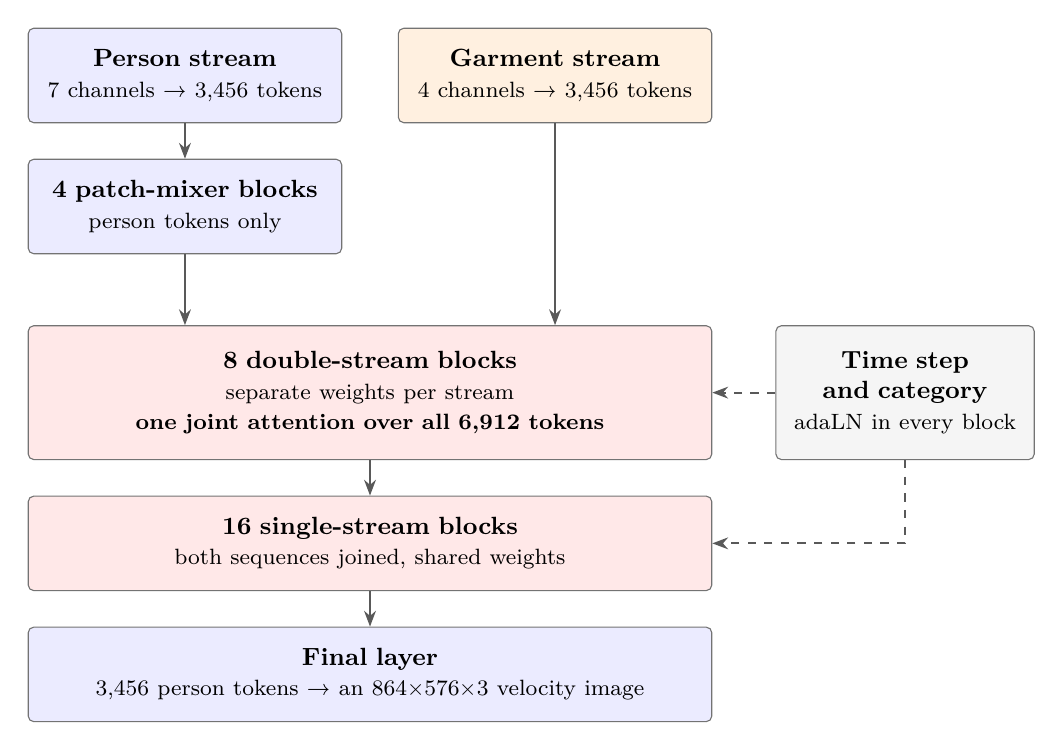
\begin{tikzpicture}[node distance=4.5mm,
  sub/.style={font=\footnotesize}]
\node[box=cB,text width=84mm,minimum height=17mm] (dbl) {\textbf{8 double-stream blocks}\\{\footnotesize separate weights per stream}\\{\footnotesize\textbf{one joint attention over all 6{,}912 tokens}}};
\node[box=cA,text width=37mm,minimum height=12mm,above=9mm of dbl.north west,anchor=south west] (mix) {\textbf{4 patch-mixer blocks}\\{\footnotesize person tokens only}};
\node[box=cA,text width=37mm,minimum height=12mm,above=of mix] (pin) {\textbf{Person stream}\\{\footnotesize 7 channels → 3{,}456 tokens}};
\node[box=cD,text width=37mm,minimum height=12mm,anchor=south east] (gin) at (pin.south -| dbl.east) {\textbf{Garment stream}\\{\footnotesize 4 channels → 3{,}456 tokens}};
\node[box=cB,text width=84mm,minimum height=12mm,below=of dbl] (sgl) {\textbf{16 single-stream blocks}\\{\footnotesize both sequences joined, shared weights}};
\node[box=cA,text width=84mm,minimum height=12mm,below=of sgl] (fin) {\textbf{Final layer}\\{\footnotesize 3{,}456 person tokens → an 864$\times$576$\times$3 velocity image}};
\node[box=black!4,text width=30mm,minimum height=17mm,right=8mm of dbl] (cond) {\textbf{Time step}\\\textbf{and category}\\{\footnotesize adaLN in every block}};
\draw[arr] (pin)--(mix); \draw[arr] (mix.south)--(mix.south|-dbl.north); \draw[arr] (gin.south)--(gin.south|-dbl.north);
\draw[arr] (dbl)--(sgl); \draw[arr] (sgl)--(fin); \draw[arr,dashed] (cond.west)--(dbl.east); \draw[arr,dashed] (cond.south)|-(sgl.east);
\end{tikzpicture}
\end{adjustbox}
\caption{The try-on transformer (an MMDiT adapted from FLUX.1). In the joint attention a token on the person's chest can read the garment token that holds the logo. Red blocks are where our LoRA adapters attach (Chapter~5).}
\label{fig:mmdit}
\end{figure}

\begin{table}[!htbp]
\centering
\caption{Layers of FASHN VTON 1.5 (hidden size 1{,}280, 10 heads of 128, MLP ratio 4).}
\label{tab:layers}
\small
\begin{tabularx}{\linewidth}{@{}L{38mm}L{12mm}Y@{}}
\toprule
\textbf{Part} & \textbf{Count} & \textbf{What it does}\\
\midrule
Patch embedders & 2 & 12$\times$12 strided convolutions; 7 and 4 input channels to 1{,}280\\
Time and category embedders & 2 & sinusoidal time embedding and a learned category table, summed\\
Patch-mixer blocks & 4 & self-attention among person tokens only\\
Double-stream blocks & 8 & per stream: modulation, QKV, output projection and a 2-layer MLP; one attention over both streams with QK-RMSNorm\\
Single-stream blocks & 16 & one fused linear layer for QKV and the MLP input, one for the output\\
Final layer & 1 & modulation and a projection back to 432 pixel values per token\\
\midrule
Total parameters & & 971{,}813{,}808 (counted on the released weights)\\
\bottomrule
\end{tabularx}
\end{table}

The joint attention of the double-stream blocks is the core of the method. Every query from a person token is compared with every key from both streams:
\begin{equation}
\operatorname{Attention}(Q, K, V) = \operatorname{softmax}\!\left(\frac{QK^\top}{\sqrt{d}}\right) V, \qquad Q, K, V \in \mathbb{R}^{6912 \times 128} \text{ per head}.
\end{equation}
A token on the person's chest can therefore place high attention weight on the garment token that holds the logo and copy what it sees. The garment is not warped or pasted; it is read.

\section{Generation by Rectified Flow}

The model is trained to predict a velocity along the straight line between a noise image $\epsilon$ and the real photograph $x_1$ (Chapter~5 derives this from the sampler). Generation integrates that velocity from noise to image with Euler steps:
\begin{equation}
x_{t+\Delta t} = x_t + \Delta t \cdot v_\theta(x_t, t, c), \qquad x_0 = \epsilon \sim \mathcal{N}(0, I).
\end{equation}
The 30 time steps are not evenly spaced. A shifted schedule with $\mu = 1.5$ spends more steps near the noise end, where the coarse layout of the image is decided.

\paragraph{Guidance} Every step runs the network on a batch of two: once with the person, garment and pose conditions and once with all of them blanked. The two velocities are combined with classifier-free guidance~\cite{cfg},
\begin{equation}
v = v_\varnothing + s\,(v_c - v_\varnothing), \qquad s = 1.5,
\end{equation}
which pushes each step towards following the garment more closely. The last step uses the conditional prediction alone, which avoids over-saturated colour at the end. One photograph therefore costs 30 network calls on a batch of two, that is 60 image passes through 972 million parameters.

\paragraph{Why colour stays true} The model has no separate colour-correction stage. Colour is preserved by three properties of the design: the garment's real pixel values enter the network directly (no VAE), guidance pulls each step towards the garment, and the unguided final step prevents over-saturation.

\section{Compute and Memory}

Table~\ref{tab:compute} summarises what the model costs to run. The operation count is our own estimate: about two operations per parameter per token for the linear layers, plus $4 L^2 d$ for attention in each of the 28 attention blocks.

\begin{table}[!htbp]
\centering
\caption{Cost of running FASHN VTON 1.5.}
\label{tab:compute}
\small
\begin{tabularx}{\linewidth}{@{}L{60mm}Y@{}}
\toprule
\textbf{Quantity} & \textbf{Value}\\
\midrule
Weights on disk (bf16) & \vBaseMb{}~MB\\
GPU memory to run (model card) & about 8~GB\\
Tokens per pass & 6{,}912\\
Attention matrix per head & 6{,}912$^2$ $\approx$ 47.8 million entries\\
Operations per photograph (estimate) & about $1.2 \times 10^{15}$\\
Hosted GPU (half an RTX Pro 6000), median of \vNRuns{} runs & \vMedTotal{}~s in total, \vMedGpu{}~s running\\
NVIDIA H100 (model card) & about 5~s\\
Our laptop (Apple M3, 8~GB) & \vGenSeconds{}~s; memory \vMemLoad{}~GB after loading, \vMemGen{}~GB after generating\\
\bottomrule
\end{tabularx}
\end{table}

The laptop figure shows why the application uses a hosted GPU: one photograph took \vGenMinutes{} minutes, roughly a hundred times longer than on the free shared GPU. To run the model at all in 8~GB we wrote a loader that keeps the weights in bf16 from the start (\vMemLoad{}~GB after loading, against 3.9~GB with FASHN's own loader) and an attention routine that processes two heads at a time instead of ten. Both reproduce FASHN's output exactly (Chapter~7).

\chapter{Proposed Work: Adapting the Model with LoRA}

\section{Overview}

FASHN VTON 1.5 was trained mostly on Western garments. Kurtis, sarees, lehengas and dupattas have drapes, borders and lengths it has rarely seen, and the sellers we built the system for sell mostly these. Improving the model for them requires fine-tuning, and fine-tuning requires three things the release does not provide: a training objective, a way to train cheaply, and paired data. This chapter describes how each was built, how the result is to be evaluated, and what adapting the model costs. Figure~\ref{fig:lorapipe} shows the whole pipeline.

\begin{figure}[!htbp]
\centering
\begin{adjustbox}{max width=\linewidth,center}
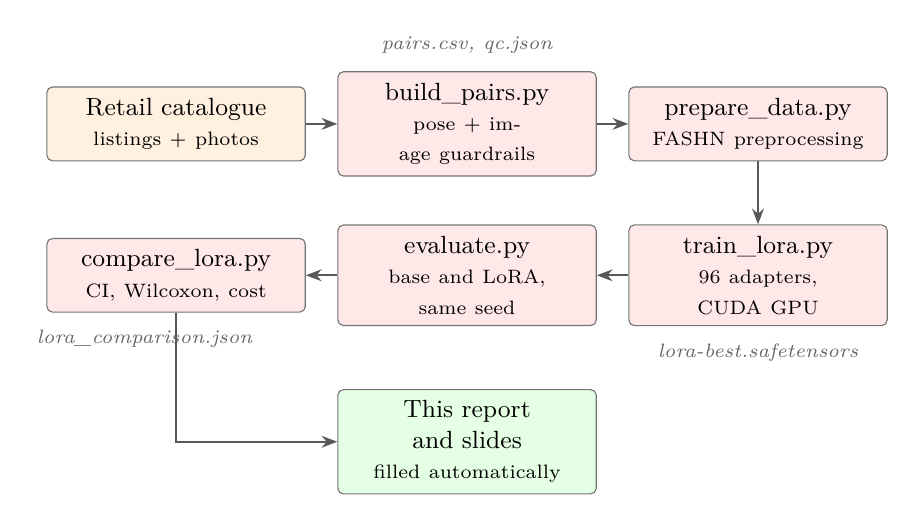
\begin{tikzpicture}[node distance=4mm]
\node[box=cD,text width=30mm] (cat) {Retail catalogue\\\scriptsize listings + photos};
\node[box=cB,text width=30mm,right=of cat] (bp) {build\_pairs.py\\\scriptsize pose + image guardrails};
\node[box=cB,text width=30mm,right=of bp] (pp) {prepare\_data.py\\\scriptsize FASHN preprocessing};
\node[box=cB,text width=30mm,below=8mm of pp] (tr) {train\_lora.py\\\scriptsize 96 adapters, CUDA GPU};
\node[box=cB,text width=30mm,left=of tr] (ev) {evaluate.py\\\scriptsize base and LoRA, same seed};
\node[box=cB,text width=30mm,left=of ev] (cp) {compare\_lora.py\\\scriptsize CI, Wilcoxon, cost};
\node[box=cC,text width=30mm,below=8mm of ev] (rep) {This report and slides\\\scriptsize filled automatically};
\draw[arr] (cat)--(bp); \draw[arr] (bp)--(pp); \draw[arr] (pp)--(tr); \draw[arr] (tr)--(ev); \draw[arr] (ev)--(cp); \draw[arr] (cp.south)|-(rep.west);
\node[note,above=1mm of bp] {pairs.csv, qc.json};
\node[note,below=1mm of tr] {lora-best.safetensors};
\node[note,below=1mm of cp,xshift=-4mm] {lora\_comparison.json};
\end{tikzpicture}
\end{adjustbox}
\caption{The adaptation pipeline, from catalogue to claimed result. Every arrow is a script in \texttt{ml/scripts}.}
\label{fig:lorapipe}
\end{figure}

\section{Reconstructing the Training Objective}

FASHN released no training code. A sampler and a training objective must agree, however, so the sampler in the released code determines the objective. Reading \texttt{\_sample} and the noise schedule gives three facts: generation starts from pure noise at $t = 0$ and ends at the image at $t = 1$; each step moves along the network's output, $x \leftarrow x + \Delta t \cdot v$; and the conditions are blanked all together for the unguided half of the batch. The only objective consistent with all three is the rectified-flow loss~\cite{rectflow,flowmatch} on the straight path from noise to the photograph:
\begin{align}
x_t &= (1 - t)\,\epsilon + t\,x_1, \qquad \epsilon \sim \mathcal{N}(0, I), \\
v^{*} &= x_1 - \epsilon, \\
\mathcal{L} &= \frac{\sum_i w_i \,\lVert v_\theta(x_t, t, c)_i - v^{*}_i \rVert^2}{\sum_i w_i}.
\end{align}
Time steps are drawn as $t = \sigma(z - \mu)$ with $z \sim \mathcal{N}(0, 1)$ and $\mu = 1.5$, which mirrors the sampler's shift towards the noise end, and with probability 0.1 all conditions are dropped together, so that guidance keeps working after fine-tuning.

\paragraph{Garment-weighted loss (our design)} We weight each pixel by
\begin{equation}
w_i = m_i \big(1 + (\lambda - 1)\, g_i\big), \qquad \lambda = 2,
\end{equation}
where $m_i$ is 0 on padding and 1 elsewhere, and $g_i$ is 1 on the garment's pixels in the target photograph. An error on the product costs twice as much as an error on the background, because for a seller a wrong print is a wrong product. This choice is untested so far; the evaluation in Section~\ref{sec:eval} can compare $\lambda = 1$ and $\lambda = 2$.

The reconstruction was confirmed in two independent ways (Chapter~7): a small model trained with this loss is sampled correctly by FASHN's unmodified sampler, and the released model has a loss \vLossRatio{} times lower under this convention than under the opposite one.

\section{LoRA Adapters}

Each adapted linear layer keeps its weight $W$ frozen and adds a low-rank path~\cite{lora}:
\begin{equation}
y = W x + \frac{\alpha}{r}\, B A x, \qquad r = 16,\ \alpha = 16,
\end{equation}
with $A$ initialised randomly and $B$ at zero, so that before training the adapted model is exactly the original one (this is one of the twelve automated tests). Table~\ref{tab:loralayers} shows where the adapters go and how the trainable parameters add up.

\begin{table}[!htbp]
\centering
\caption{Placement of the LoRA adapters ($r = 16$). Trainable parameters of one adapter: $r\,(d_\text{in} + d_\text{out})$.}
\label{tab:loralayers}
\small
\begin{tabularx}{\linewidth}{@{}L{28mm}YL{17mm}r@{}}
\toprule
\textbf{Blocks} & \textbf{Layers wrapped (each stream)} & \textbf{Adapters} & \textbf{Parameters}\\
\midrule
8 double-stream & QKV 1280→3840, output 1280→1280, MLP 1280→5120, MLP 5120→1280; person and garment stream & 8 × 8 = 64 & 5{,}242{,}880\\
16 single-stream & fused \texttt{linear1} 1280→8960, \texttt{linear2} 6400→1280 & 16 × 2 = 32 & 4{,}587{,}520\\
\midrule
Total & \vLoraLayers{} & \vTrainParams{}\\
\bottomrule
\end{tabularx}
\end{table}

\noindent The \vTrainParams{} trainable parameters are \vLoraPct{}\% of the model. The double-stream blocks were chosen because they are where garment detail is transferred to the body (Figure~\ref{fig:mmdit}), which is where knowledge of a new kind of garment has to go.

Three decisions are specific to this model:
\begin{enumerate}
\item \textbf{Adapters in float32 over a bf16 model.} bf16 has an 8-bit mantissa; the small updates of early training vanish when added to a bf16 weight, so the adapters are kept and trained in float32.
\item \textbf{Modulation layers stay frozen.} They turn the time step into the scale and shift of every block, so changing them would change the behaviour of every sampling step at once.
\item \textbf{One adapter on the fused layer.} In single-stream blocks one linear layer computes both the attention inputs and the MLP input, so one adapter covers both.
\end{enumerate}

\paragraph{New garment categories} The category embedding has four rows. The function \texttt{extend\_\allowbreak categories} adds rows, for example saree as category~4 and lehenga as category~5, each initialised as a copy of ``one-pieces'', so that existing categories are unchanged (another automated test) and the new one starts from the nearest known behaviour.

\section{Running the Model in 8~GB}

The project's only machine was an Apple M3 laptop with 8~GB of memory, so the training code had to run there for development:
\begin{itemize}
\item a loader that builds the network on the meta device and loads the weights directly in bf16 (\vMemLoad{}~GB after loading, against 3.9~GB with FASHN's loader);
\item attention computed two heads at a time instead of ten, which bounds the peak memory of the $6{,}912^2$ attention matrix;
\item rotary embeddings in float32 on Apple GPUs, which lack float64 (shown equal to FASHN's float64 version by a test);
\item gradient checkpointing~\cite{checkpoint}, which recomputes block activations during the backward pass.
\end{itemize}
Even so, a full-resolution training step did not fit: it filled memory and 8.6~GB of swap and did not finish one step in eight minutes. Training at full resolution needs a CUDA GPU with at least 16~GB.

\section{From a Retail Catalogue to Training Pairs}
\label{sec:pairs}

\subsection{What a pair is}

Each training example needs two photographs of the \emph{same} product: one of a person wearing it (the target the model must learn to produce) and one of the garment alone, either flat-lay or on a mannequin, or else worn in a different photograph. A product listing usually contains both kinds: a model shot from the front, and a product shot on a plain background. The listings are not labelled, however, and many photographs are back views, close-ups of a collar or a print, fabric swatches, or shared between several colour variants. Any of these, used as a training pair, would teach the model something wrong.

\subsection{Pose and image guardrails}

\texttt{build\_pairs.py} runs every photograph through FASHN's own person detector and pose estimator, and applies the rules in Table~\ref{tab:guard}. Each rule was added because a test run on a sample of the catalogue produced exactly the failure it prevents; Chapter~7 shows the resulting pairs.

\begin{table}[!htbp]
\centering
\caption{Guardrails applied to catalogue photographs.}
\label{tab:guard}
\small
\begin{tabularx}{\linewidth}{@{}L{48mm}Y@{}}
\toprule
\textbf{Rule} & \textbf{Failure it prevents}\\
\midrule
\multicolumn{2}{@{}l}{\textit{Every photograph}}\\
Short side $\ge$ 384~px; sharpness (variance of the Laplacian~\cite{laplacian} at 512~px) $\ge$ 12 & unusably small or blurred photographs\\
Perceptual hash: a photograph is used by one product only & colour variants sharing photos, which would pair a red product's photo with a blue one\\
\multicolumn{2}{@{}l}{\textit{Target photograph (person wearing the product)}}\\
Detector confidence $\ge$ 0.6 & the pose model ``finding'' a body in a print close-up\\
One dominant person (a second one under 35\% of its height) & group shots\\
Shoulders and hips visible and inside the frame & collar close-ups (the pose model guesses joints beyond the frame)\\
Knees visible, for bottoms and one-pieces & cropped legs\\
Face visible and body facing the camera (the person's left shoulder on the right of the photo) & back views; the face score alone is unreliable, the left--right order is not\\
Shoulder width $\ge$ 0.45 × torso height; person $\ge$ 45\% of the photo height & side views and distant shots\\
\multicolumn{2}{@{}l}{\textit{Garment-only photograph}}\\
Plain, light border that differs from the centre; product touching at most two edges & fabric swatches and print close-ups that fill the frame\\
\multicolumn{2}{@{}l}{\textit{Worn photograph used as the garment input}}\\
Same front-view rules as a target & back views hiding the front of the garment\\
\bottomrule
\end{tabularx}
\end{table}

\subsection{Pairing and splitting}

For each product the best target is the passing worn photograph with the most visible keypoints, the largest person and the highest sharpness. The garment input is the sharpest garment-only photograph (photo type \emph{flat-lay}); if there is none, a second passing front-view photograph (photo type \emph{model}). Products without a usable target or a usable garment photograph are skipped and counted, and products with fewer than two photographs on disk are skipped before any analysis, because most listings carry only their main photograph. The split into training and validation is made by product family (the parent listing that groups colour and size variants), using a hash of the family identifier, so no garment can appear on both sides; the script verifies this and reports the overlap, which must be zero~\cite{leakage}. All decisions are cached per photograph, so a long run can be resumed, and summarised in \texttt{qc.json}.

\section{Training Configuration}

Pairs are prepared with FASHN's own preprocessing in \emph{masked} mode: the human parser greys out the garment region of the person photograph and the model learns to fill it with the garment, which is how FASHN describes the first stage of its own training. The second stage, segmentation-free ``triplets'' in which the base model first dresses the person in a different garment, needs one generation per sample and therefore a CUDA GPU; \texttt{prepare\_data.py --triplets} implements it for the full run.

\begin{table}[!htbp]
\centering
\caption{Training configuration (\texttt{haat\_ft/train.py}).}
\label{tab:traincfg}
\small
\begin{tabularx}{\linewidth}{@{}L{55mm}Y@{}}
\toprule
\textbf{Setting} & \textbf{Value}\\
\midrule
Adapter rank, scale & $r = 16$, $\alpha = 16$, on attention and MLP layers\\
Optimiser & AdamW~\cite{adamw}, learning rate $10^{-4}$, weight decay 0.01\\
Schedule & 100 warm-up steps, then cosine decay to 10\%\\
Batch & 1 with 4 accumulation steps (effective 4)\\
Steps & 2{,}000 (validation every 200, best adapter kept)\\
Condition dropout & 0.1, all conditions together\\
Garment weight $\lambda$ & 2\\
Gradient clipping & 1.0\\
Memory & gradient checkpointing; bf16 base, float32 adapters\\
\bottomrule
\end{tabularx}
\end{table}

\section{Evaluation Protocol}
\label{sec:eval}

The base model and the adapted model are run on every validation pair with the same inputs, the same seed and the same sampler settings (30 steps, guidance 1.5), and each output is compared with the real photograph:
\begin{itemize}
\item \textbf{PSNR} over the unpadded image (higher is better);
\item \textbf{SSIM}~\cite{ssim} over the unpadded image (higher is better);
\item \textbf{garment L1}: the mean absolute error on the garment's pixels only, the number a seller cares about (lower is better);
\item generation time for each model;
\item \textbf{model guardrails} (\texttt{guardrail\_eval.py}): \emph{pose drift}, the mean distance between the body keypoints of the output and of the real photograph found by FASHN's own pose estimator, as a fraction of the image diagonal; \emph{garment colour error}, the CIEDE2000 palette distance $D$ ($k_L = 2$, Section~\ref{sec:colour}) between the garment's pixels in the output and in the real photograph; and blank or unchanged outputs. Palettes are used instead of pixel-by-pixel differences, which punish a fold that moved by a few pixels even when every colour is right. An output passes the guardrail when it is neither blank nor unchanged, its pose drift is at most 0.05 and its colour error at most 12, the ``same shade'' limit of Table~\ref{tab:tolerance}; the pass rate of each model is reported.
\end{itemize}
For each metric \texttt{compare\_lora.py} computes the paired difference (adapter minus base), its 95\% bootstrap confidence interval over 10{,}000 resamples of the validation garments~\cite{bootstrap}, the share of garments on which the adapter is better, and a two-sided Wilcoxon signed-rank test~\cite{wilcoxon} (exact for up to 25 garments).

\paragraph{When an improvement may be claimed} An improvement is reported only when the 95\% confidence interval of the difference excludes zero in the favourable direction \emph{and} the Wilcoxon test gives $p < 0.05$. With fewer than six garments the Wilcoxon test cannot reach that level, so very small comparisons can never claim an improvement. Otherwise the result is reported as ``no clear change'' or ``worse''. Because pixel metrics can miss a wrong logo, the side-by-side images (inputs, real photograph, base, adapter) are kept for every garment and a sample is shown in the report. A rubric score by two human raters, blind to which model produced which image, is planned on top of these numbers.

\section{Compute Cost of the Adaptation}

LoRA does not make the model cheaper to \emph{run}: a photograph still needs 60 passes through all 972 million parameters, and an unmerged adapter adds roughly one per cent to the work of the layers it wraps. Merged into the weights after training, it adds nothing. What LoRA makes cheaper is \emph{training} and \emph{shipping} the change (Table~\ref{tab:cost}).

\begin{table}[!htbp]
\centering
\caption{Cost of adapting the model: full fine-tuning against LoRA. Training state counts weights, gradients and the two AdamW moments; activations are excluded because they are the same for both and are reduced by checkpointing.}
\label{tab:cost}
\small
\begin{tabularx}{\linewidth}{@{}L{55mm}YY@{}}
\toprule
& \textbf{Full fine-tuning} & \textbf{LoRA (ours)}\\
\midrule
Trainable parameters & 971.8M (100\%) & \vTrainParamsM{}M (\vLoraPct{}\%)\\
Training state in memory & \vFullStateGb{}~GB (16 bytes per parameter) & \vLoraStateGb{}~GB (bf16 base + float32 adapters)\\
File to store or ship & \vBaseMb{}~MB & \vAdapterMb{}~MB (\vAdapterPct{}\%)\\
Effect on a 972M model trained on $\sim$18M pairs, given a few hundred new pairs & likely to overwrite general knowledge & base frozen; adapter can be removed\\
Inference cost & unchanged & unchanged when merged\\
\bottomrule
\end{tabularx}
\end{table}

\noindent The training state shrinks by a factor of about \vStateRatio{}, which is what makes a single 16~GB GPU sufficient. Figure~\ref{fig:compute} shows the same comparison.

\begin{figure}[!htbp]
\centering
\includegraphics[width=0.92\linewidth]{compute.pdf}
\caption{Memory needed for the training state, and the size of what has to be stored, for full fine-tuning and for LoRA.}
\label{fig:compute}
\end{figure}

\section{How a Photograph Will Be Produced after Integration}
\label{sec:integration}

Figure~\ref{fig:integration} shows how a request will flow once the adapter is part of the application, and Table~\ref{tab:layers-after} what each layer contributes before and after. The integration needs no change to the orchestration: an engine is one file plus one line in the registry (Section~3.5).

\begin{figure}[!htbp]
\centering
\begin{adjustbox}{max width=\linewidth,center}
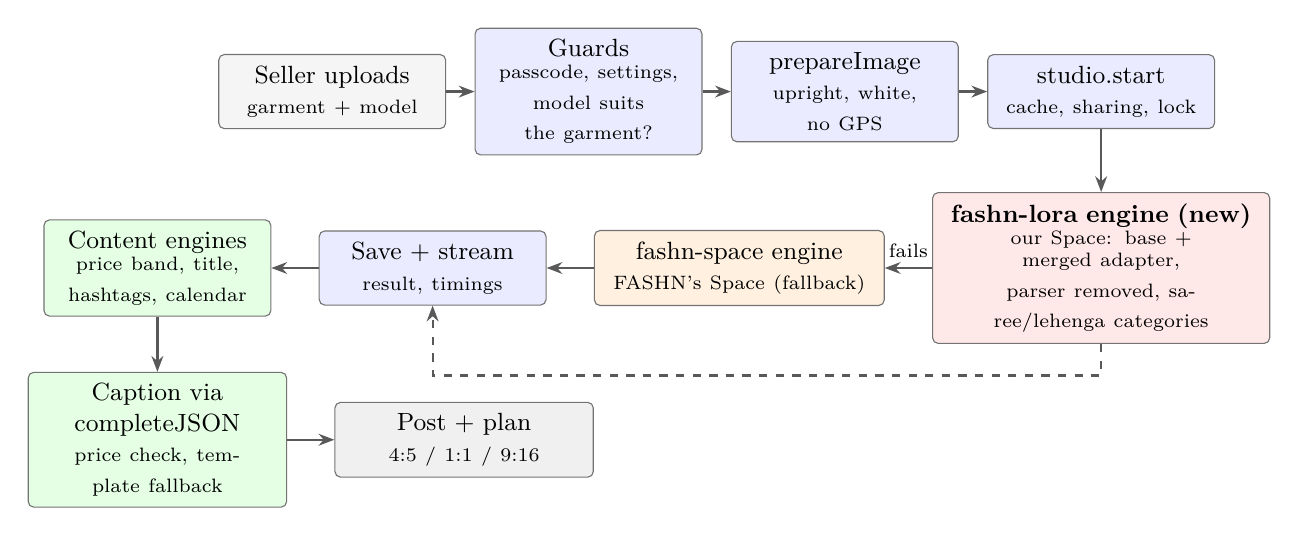
\begin{tikzpicture}[node distance=3.6mm]
\node[box,text width=26mm] (u) {Seller uploads\\\scriptsize garment + model};
\node[box=cA,text width=26mm,right=of u] (g) {Guards\\\scriptsize passcode, settings,\\model suits the garment?};
\node[box=cA,text width=26mm,right=of g] (c) {prepareImage\\\scriptsize upright, white, no GPS};
\node[box=cA,text width=26mm,right=of c] (s) {studio.start\\\scriptsize cache, sharing, lock};
\node[box=cB,text width=40mm,below=8mm of s] (l) {\textbf{fashn-lora engine (new)}\\\scriptsize our Space: base + merged adapter,\\parser removed, saree/lehenga categories};
\node[box=cD,text width=34mm,left=6mm of l] (f) {fashn-space engine\\\scriptsize FASHN's Space (fallback)};
\node[box=cA,text width=26mm,left=6mm of f] (v) {Save + stream\\\scriptsize result, timings};
\node[box=cC,text width=26mm,left=6mm of v] (e) {Content engines\\\scriptsize price band, title,\\hashtags, calendar};
\node[box=cC,text width=30mm,below=7mm of e] (cap) {Caption via completeJSON\\\scriptsize price check, template fallback};
\node[box=black!6,text width=30mm,right=6mm of cap] (post) {Post + plan\\\scriptsize 4:5 / 1:1 / 9:16};
\draw[arr] (u)--(g); \draw[arr] (g)--(c); \draw[arr] (c)--(s); \draw[arr] (s)--(l); \draw[arr] (l)--node[above,font=\scriptsize]{fails}(f); \draw[arr] (f)--(v); \draw[arr] (v)--(e); \draw[arr] (e)--(cap); \draw[arr] (cap)--(post);
\draw[arr,dashed] (l.south) |- ++(0,-4mm) -| (v.south);
\end{tikzpicture}
\end{adjustbox}
\caption{The request path after integration. The adapted model is tried first; FASHN's own Space remains the fallback; the content engines turn the result into a post.}
\label{fig:integration}
\end{figure}

\begin{table}[!htbp]
\centering
\caption{What each layer of the system contributes now and after integration.}
\label{tab:layers-after}
\small
\begin{tabularx}{\linewidth}{@{}L{30mm}YY@{}}
\toprule
\textbf{Layer} & \textbf{Now (base model)} & \textbf{After integration}\\
\midrule
Input guards & passcode, settings, photo cleaning, model-suitability marks & same, plus garment-photo checks (blur, cut-off garment) before any GPU time\\
Orchestration & cache, job sharing, GPU lock, error chain & unchanged; the chain gains a second real engine\\
Try-on network & FASHN VTON 1.5 as released, on FASHN's Space & same network with the merged LoRA adapter on our own Space; categories 0--3 plus saree and lehenga\\
Licence & human parser loaded although unused & parser removed: the whole pipeline is Apache-2.0\\
Inference cost & 60 passes, $\sim$\vMedTotal{}~s on the free GPU & identical (a merged adapter adds no computation)\\
Fallback & none in practice (one real engine) & FASHN's Space if our Space is down or out of quota\\
Content & captions and research report & plus catalogue-driven price band, title, hashtags, positioning and calendar\\
Evaluation & rubric on 4 images & base-vs-adapter comparison with confidence intervals on held-out garments (Section~\ref{sec:e6}), repeated for each new adapter\\
\bottomrule
\end{tabularx}
\end{table}

\section{Summary of Experiments}

\begin{table}[!htbp]
\centering
\caption{Experiments of this project and their status.}
\label{tab:experiments}
\small
\begin{tabularx}{\linewidth}{@{}L{8mm}YL{30mm}L{18mm}@{}}
\toprule
\textbf{ID} & \textbf{Question} & \textbf{Data} & \textbf{Status}\\
\midrule
E1 & Does our inference code reproduce FASHN's output exactly? & real weights, 1 pair & done\\
E2 & Is the reconstructed objective the one the model was trained with? & real weights; tiny model & done\\
E3 & Does the human parser affect the output in our mode? & real weights & done\\
E4 & Does the training loop work on the real network? & 2 + 1 pairs, half resolution & done\\
E5 & How many usable pairs does the catalogue give, and why are photos rejected? & retail catalogue & \ifPairs done\else running\fi\\
E6 & Does the adapter improve held-out garments, and by how much? & catalogue pairs, CUDA GPU & \ifLora done\else pending\fi\\
\bottomrule
\end{tabularx}
\end{table}

\chapter{Market Intelligence and Content Engines}

\section{Overview}

A try-on photograph sells nothing on its own. The seller still needs a caption, a price, a title buyers will search for, hashtags and a sense of when to post. This chapter describes the part of the system that produces them. It rests on one principle: \emph{language models write words, code computes numbers}. Language models are good at tone and phrasing and unreliable at arithmetic, prices and dates, so every number a seller sees is computed by code from the seller's own answers or from catalogue statistics, and every model answer is validated before use.

The chapter has two halves. Sections~\ref{sec:llm}--\ref{sec:research} describe what runs in the application today: the text-AI layer, captions and the market-research report. Sections~\ref{sec:catalogue}--\ref{sec:engines} describe the catalogue analysis and the content engines built on it, which run as a Python module (\texttt{analysis/market.py}) and are not yet connected to the application's screens.

\section{One Validated Function for All Text AI}
\label{sec:llm}

Every call to a language model in the application goes through one function, \texttt{completeJSON(\allowbreak schema, request)}. It receives a prompt and a zod schema that describes the exact shape the answer must have, and tries the providers listed in \texttt{LLM\_CHAIN} in order:

\begin{enumerate}
\item skip a provider whose API key is not set;
\item send the request to its OpenAI-compatible \texttt{/chat/completions} endpoint in JSON mode, with a 45-second timeout;
\item extract the JSON object from the reply, removing Markdown fences and any text around it;
\item validate it against the schema; a wrongly shaped answer counts as a failure, exactly like a network error;
\item return the data and the name of the model that produced it, or record the failure and try the next provider.
\end{enumerate}

\noindent If every provider fails, the function raises \texttt{LlmUnavailable} with the list of all attempts, and the caller falls back to a template built only from the seller's own input, clearly labelled as such. The default chain is Groq's Llama~3.3~70B~\cite{groq} followed by Gemini~2.5~Flash~\cite{gemini}; both are free and speak the same API, so one code path serves both. In our deployment only the Gemini key is configured, so Groq is skipped and every AI-written text so far came from Gemini~2.5~Flash, at about 9~s per research report.

One problem found in testing shows why such details matter: Gemini~2.5~Flash spends its output budget on hidden ``thinking'' and returned empty answers to short requests. The function therefore sends \texttt{reasoning\_effort: "none"} to Gemini only (other providers reject the field).

\section{Captions}

A caption request carries the product name, price, MRP, offer line, call to action, tone and language (English, Hinglish or Hindi), and optionally the seller's saved research report. Three rules protect the seller:

\begin{enumerate}
\item \textbf{No invented prices.} \texttt{pricesMentioned()} finds every rupee amount in the caption, written as \rupee, Rs, INR or {\devafont रु}, including Devanagari digits. If any amount differs from the seller's price and MRP, the answer is rejected and the next provider (or the template) is used. A caption that omits the price gets it appended.
\item \textbf{Hashtags in English letters.} Shoppers search \texttt{\#cottonkurti}, not its Devanagari spelling. This rule had to be placed in the system prompt; in the user prompt alone the model ignored it.
\item \textbf{The template claims nothing.} Without a working model the caption uses only the fields the seller typed.
\end{enumerate}
\noindent Hashtags are cleaned (de-duplicated case-insensitively, capped at 30, Instagram's limit).

\section{The In-App Research Report}
\label{sec:research}

The research report answers ten questions the seller fills in once (product, city, price range, cost per piece, buyers, goal and channels). It deliberately combines three sources:

\begin{enumerate}
\item \textbf{The seller's own answers}, validated by a zod schema; a mistake returns a list of the wrong fields.
\item \textbf{Facts computed in code.} Profit and margin per piece,
\begin{equation}
\text{profit} = p - c, \qquad \text{margin} = \operatorname{round}\!\left(100 \cdot \frac{p - c}{p}\right)\%,
\end{equation}
at both ends of the seller's price range, with a ``loss'' warning when the profit at the lowest price is not positive and a ``thin'' warning below 30\%; and the selling occasions (festivals, sale weekends) in the next 75 days, from a fixed list of dates in the code. Festivals that follow the lunar calendar are left out rather than risk a wrong date.
\item \textbf{The language model's general knowledge}: buyer persona, trends, content ideas, a seven-day plan, hashtags and risks. The model is told it has no internet access and must not invent statistics, follower counts or brand names, and the report says so to the seller.
\end{enumerate}

\noindent Warnings are stored as codes (for example \texttt{\{code: "thin", pct: 20\}}), not as sentences, so one saved report can be shown in English or Hindi. Reports are written to a temporary file and renamed into place, so a crash never leaves a broken file.

\section{Catalogue Analysis}
\label{sec:catalogue}

The in-app report has no live market data. To give the content engines real numbers, we analysed a retail catalogue of \ifMarket\vMkTotalRaw{}\else about 280{,}000\fi{} listings from two marketplaces: men's T-shirts and women's tops from Amazon.in, and sarees and kurta sets from Myntra. Each listing has a selling price, MRP, discount, average star rating, number of ratings, brand, title and structured attributes (colour, fabric, neck, sleeve, pattern and fit for the Western categories; fabric, border, ornamentation and weave for sarees; pattern, neck and sleeve for kurta sets). The catalogue was collected from public product pages in October 2026 and is used here only for non-commercial academic analysis; no listing or photograph is redistributed with this report.

\subsection{Cleaning}

\begin{enumerate}
\item \textbf{One listing per product family.} Colour and size variants share one parent listing and usually share its ratings; counting each variant would multiply the same demand. The variant with the most ratings represents the family.
\item \textbf{Outlier prices.} Prices outside $[Q_1 - 3\,\mathrm{IQR},\ Q_3 + 3\,\mathrm{IQR}]$ are removed and counted.
\item \textbf{Attribute spellings.} ``100\% Cotton'', ``Pure Cotton'' and ``Cotton'' become \emph{Cotton}; ``Crew Neck'' and ``Round Neck'' become \emph{Round/crew}; ``Art Silk'', ``Silk Blend'' and ``Pure Silk'' stay distinct because they sell at different prices; and so on for every attribute. Myntra listings flagged with a scraping error are dropped.
\end{enumerate}

\subsection{The demand signal}

Units sold are not in the data. The number of ratings is visible and grows with sales~\cite{wom}, so it serves as the demand signal. Raw counts are dominated by a few bestsellers (in the women's tops a single listing holds \ifMarket\vMkTopTopOne\else a large share\fi{}\% of all ratings), so shares and lifts use a damped weight,
\begin{equation}
D(\ell) = \log\big(1 + n_\text{ratings}(\ell)\big),
\end{equation}
while totals use raw counts. A lifetime unit estimate is given only as a range, assuming that 1--3\% of buyers leave a rating; this rate is an assumption, not a measured value, and the range should be read as an order of magnitude.

\subsection{Measures}

\begin{itemize}
\item \textbf{Price tiers}: value, mid and premium, cut at the 33rd and 67th price percentiles, with each tier's share of listings and of demand.
\item \textbf{Attribute lift}: for an attribute value $a$,
\begin{equation}
\text{lift}(a) = \frac{\sum_{\ell : a} D(\ell) \,/\, \sum_\ell D(\ell)}{\left|\{\ell : a\}\right| / |\{\ell\}|},
\end{equation}
the share of demand over the share of listings. A lift above 1 means buyers want more of it than sellers offer; values with fewer than five listings are not reported.
\item \textbf{Concentration}: the demand share of the ten largest brands and the Herfindahl--Hirschman index $\mathrm{HHI} = 10^4 \sum_b s_b^2$.
\item \textbf{Associations}: Spearman rank correlations~\cite{spearman} between price, discount, star rating and number of ratings.
\item \textbf{Search keywords}: title words and word pairs, brand names removed, scored by $\sum D(\ell)$ over the listings that use them.
\end{itemize}

\section{Content Engines}
\label{sec:engines}

Five engines turn these statistics into advice for one seller. They take the seller's category, attributes, cost, city and date, and every number they output comes from the catalogue statistics. Chapter~7 runs them on a worked example.

\paragraph{Pricing engine} Comparable listings are those in the same category that match the seller's product on at least two of fabric, neck, sleeve, pattern and fit (at least 15 are required, otherwise the 30 closest are used). The engine reports their 25th, 50th and 75th price percentiles and recommends the band between the 40th and 60th percentiles, which places the seller in the middle of comparable products. It computes the margin at both ends of the band from the seller's cost, the lowest price that keeps a 30\% margin, $\lceil c / 0.7 \rceil$, and the tier the band falls in. It never suggests raising the MRP to make a discount look larger, although the median catalogue discount (above 50\%) shows how common that practice is.

\paragraph{Title (SEO) engine} The product title is assembled from the seller's real attributes in the order buyers search for them (shop, audience, fabric and pattern, product, then neck, sleeve and fit), written in shoppers' words (``Round Neck'', ``3/4 Sleeve''). Its length is compared with the median title length of the best-selling quarter of listings, and the engine lists words that the best-selling comparable listings use and the title does not, to be added only if true.

\paragraph{Hashtag engine} Tags come in four tiers: broad (the product noun and small-business tags), niche (attribute plus product, such as \texttt{\#embroideredtop}), local (the city) and occasion (the next selling moments). Two-word search keywords become tags only when they match the seller's own attributes, so a tag never claims a fabric or a feature the product does not have. Tags are in English letters, de-duplicated and capped at 30.

\paragraph{Positioning and demographics} The engine states the audience (from the category's gender and the seller's channels), the tier, a one-sentence positioning statement that quotes the comparable median price, the most demanded value of each attribute, and the attributes with the highest lift.

\paragraph{Location engine (GEO)} Here GEO means geographic targeting: local hashtags for the seller's city and the selling moments in the next 75 days from the same dated calendar the research report uses. The catalogue itself carries no location, so regional demand cannot yet be measured; this is listed as future work.

\paragraph{Hooks and description} The first line of a caption is what a buyer sees before ``more''. The rules are: lead with the product and the occasion rather than the brand, put the price in the caption, state one benefit the seller can prove (fabric, fit), and end with the call to action. The description is built from the same attribute facts as the title.

\section{The Engines Inside the Application}
\label{sec:engines-app}

The engines above run inside the application, not only in the analysis script. \texttt{analysis/market.py --app-out} writes a compact catalogue for the application: per category the statistics of Section~\ref{sec:engines} and a fixed random sample of 6{,}000 listings as numbers only (price, ratings, stars, discount and attribute codes; no titles, brands, links or photographs). The application's \texttt{src/lib/market} is a line-by-line port of the engines with the same quantile function, checked by automated tests against a synthetic catalogue.

The research questionnaire gains an optional step, \emph{Compare with real listings}, where the seller picks the product type (T-shirt, top, saree or kurta set) and its attributes in the catalogue's own spelling. The report then shows a \emph{From real listings} section with the recommended price band, the margin at the seller's cost, the 30\%-margin floor, a listing title built only from the seller's attributes, the demand words the title lacks, the hashtags and the positioning statement. The same numbers are given to the language model with the instruction not to contradict them and to keep its price range inside the comparable listings' interquartile range. For the worked example of Section~\ref{sec:engines}, the application's sample gave a band of \rupee1,449--\rupee1,577 against \rupee1,449--\rupee1,578 from the full catalogue, and Gemini~2.5 Flash, given these numbers, recommended exactly \rupee1,449--\rupee1,577. Without a catalogue file the step is simply switched off.

\section{Guardrails of the Content Side}

\begin{table}[!htbp]
\centering
\caption{What could go wrong in generated text, and the rule that prevents it.}
\label{tab:textguard}
\small
\begin{tabularx}{\linewidth}{@{}L{55mm}Y@{}}
\toprule
\textbf{Risk} & \textbf{Rule}\\
\midrule
A model invents a price or an offer & any rupee amount other than the seller's price or MRP rejects the answer\\
Wrong arithmetic or wrong dates & margins, bands and calendars are computed in code; models never see the task\\
Malformed or partial answers & zod validation; a bad shape is a failure and the next provider is tried\\
A provider is down or out of free quota & provider chain, then a labelled template; the seller is told which one wrote the text\\
Made-up market statistics & the prompt forbids them; real statistics come only from the catalogue analysis\\
Hashtags in a script buyers do not search & English letters only, enforced in the system prompt and in code\\
Tags or titles claiming features the product lacks & tags and titles are built from the seller's own attributes\\
Inflated MRP to show a large discount & the engine never proposes an MRP\\
A single bestseller dominating the statistics & log-damped demand, a minimum of five listings per reported value\\
\bottomrule
\end{tabularx}
\end{table}

\chapter{Results and Discussion}

\section{Experimental Setup}

\paragraph{Software environment and reproducibility} The application runs on Node.js with Next.js~16 and TypeScript; the model work runs on Python~3.12 with PyTorch and FASHN's \texttt{fashn-vton} 1.5.0 package; the pose guardrails use FASHN's own ONNX detector and pose estimator through ONNX Runtime. Every number in this chapter is read by the report's build script from a result file written by the project's scripts (Appendix~A); none is typed by hand.

\paragraph{Hardware} Development and all local experiments ran on an Apple M3 laptop with 8~GB of unified memory. Hosted generations ran on Hugging Face ZeroGPU, which assigns half of an NVIDIA RTX Pro 6000 (48~GB) per call. The LoRA comparison (Section~\ref{sec:e6}) requires a CUDA GPU with at least 16~GB.

\paragraph{Real and estimated results} All results are measured on real data unless a sentence says ``estimate''. The unit-sales range of Section~\ref{sec:market} rests on an assumed rating rate, and the compute cost of Table~\ref{tab:cost} is computed from parameter counts.

\section{Serving the Model}

\subsection{Time per photograph}

Figure~\ref{fig:timing} shows all \vNRuns{} real generations made through the application on 26--27 October 2026. The median time from request to finished image was \vMedTotal{}~s, of which \vMedGpu{}~s was spent running on the GPU (including the download of the result) and \vMedQueue{}~s waiting in the Space's queue. Two runs took only \vMinTotal{}~s; the shared GPU's speed varies and we cannot see why from outside.

\begin{figure}[!htbp]
\centering
\includegraphics[width=0.9\linewidth]{timing.pdf}
\caption{Time for each of the \vNRuns{} real generations, split into queue time and GPU time (FASHN VTON 1.5 on Hugging Face ZeroGPU, 30 steps).}
\label{fig:timing}
\end{figure}

\subsection{The cache}

A repeat request with the same photographs and settings is answered without the GPU. We measured the server-side path (photograph check, key computation and disk look-up) 25 times on the saved T-shirt result: the median was \vCacheMs{}~ms, about \vCacheRatio{} times faster than a new photograph (Figure~\ref{fig:cache}). The page tells the seller that no GPU was used (Figure~\ref{fig:saved}).

\begin{figure}[!htbp]
\centering
\includegraphics[width=0.7\linewidth]{cache.pdf}
\caption{Time to answer a repeat request from the cache against a new generation.}
\label{fig:cache}
\end{figure}

\begin{figure}[!htbp]
\centering
\includegraphics[width=0.55\linewidth]{shot-saved.png}
\caption{What the seller sees on a repeat request (screenshot of the running application).}
\label{fig:saved}
\end{figure}

\subsection{The free GPU quota}

Figure~\ref{fig:quota} shows how many photographs remain after each one, by time and by run count. With \vPerPhoto{}~s per photograph and 60~s reserved for each call, the time budget allows \vByTimeFresh{} photographs a day, but the run limit is reached first: on 26 October the Space refused our ninth photograph after only \vUsedAtRefusal{}~s of GPU time, with a ``runs limit'' message. The ledger learned the limit (\vRunsLimit{}) from that message, and the application has shown ``about \vRunsLimit{} photos left'' since.

\begin{figure}[!htbp]
\centering
\includegraphics[width=0.75\linewidth]{quota.pdf}
\caption{Photographs left in the day after each photograph made, limited by GPU time and by the learned run limit.}
\label{fig:quota}
\end{figure}

\section{Output Quality Baseline}

Four try-ons were scored on six criteria from 1 (wrong) to 5 (indistinguishable from the product): colour, print, neckline or waist, sleeves or length, shape and fit, and absence of artefacts (Figure~\ref{fig:rubric}, Table~\ref{tab:rubric}). The scores were given from full-size crops by an AI assistant and have not yet been confirmed by a human rater, so they are a first baseline, not a benchmark.

\begin{figure}[!htbp]
\centering
\includegraphics[width=0.92\linewidth]{rubric.pdf}
\caption{Rubric scores of the four baseline try-ons (30 points each).}
\label{fig:rubric}
\end{figure}

\begin{table}[!htbp]
\centering
\caption{Baseline try-ons (balanced quality, 30 steps, seed 42, flat-lay garments).}
\label{tab:rubric}
\small
\begin{tabularx}{\linewidth}{@{}L{32mm}L{38mm}cY@{}}
\toprule
\textbf{Garment} & \textbf{Model wearing} & \textbf{Score} & \textbf{Note}\\
\midrule
Black logo T-shirt & T-shirt and chinos & 30/30 & logo text reproduced exactly\\
Navy eyelet crop top & dress & 28/30 & lace kept on the sleeves, body smoothed\\
White tiered skirt & dress & 11/30 & skirt blended into the dress\\
White tiered skirt & T-shirt and shorts & 29/30 & dot pattern and waistband kept\\
\bottomrule
\end{tabularx}
\end{table}

\begin{figure}[!htbp]
\centering
\includegraphics[width=0.95\linewidth]{baseline-sheet.jpg}
\caption{Baseline try-ons. Columns: garment, model photograph, result.}
\label{fig:sheet}
\end{figure}

\paragraph{The skirt lesson} The model replaces clothing. A skirt replaces a bottom garment, and a model wearing a dress has no separate bottom to replace, so in segmentation-free mode the skirt merged into the dress. The same skirt on a model in a T-shirt and shorts scored 29/30 (Figure~\ref{fig:skirt}). We changed the application, not the model: every preset model now records what it is wearing and which garment types it suits, and the studio marks each model with a tick or a cross for the chosen category. This raised the score of this garment from 36.7\% to 96.7\%. It is the only measured improvement in output quality in this report, it came from how the model is used, and it rests on one garment.

\begin{figure}[!htbp]
\centering
\includegraphics[width=0.75\linewidth]{skirt.jpg}
\caption{The tiered skirt on a model wearing separates (29/30).}
\label{fig:skirt}
\end{figure}

\section{Checks on the Real Weights (E1--E3)}

\paragraph{E1: our inference code equals FASHN's} With our loader, our chunked attention and our float32 rotary embeddings, the output of the full pipeline differs from FASHN's own pipeline by a mean of \vEquivDiff{} out of 255 (PSNR 148~dB, numerically identical).

\paragraph{E2: the reconstructed objective} Figure~\ref{fig:recon} shows the loss of the released, untouched model on a real pair at five time steps, under our convention and under the reversed one. Under ours the mean loss is \vLossOurs{}; under the reversed convention it is \vLossRev{}, \vLossRatio{} times higher. A trained model has a low loss only under the convention it was trained with, so this identifies the objective. Independently, a small model trained from scratch with our loss is sampled correctly by FASHN's unmodified sampler (error 0.80 → 0.005), while the reversed convention makes it worse (0.80 → 1.14).

\begin{figure}[!htbp]
\centering
\includegraphics[width=0.75\linewidth]{recon.pdf}
\caption{Loss of the pretrained model under the reconstructed and the reversed time convention (log scale).}
\label{fig:recon}
\end{figure}

\paragraph{E3: the human parser is not needed in our mode} Replacing the human parser with a stub changes the output by \vParserDiff{} out of 255 in segmentation-free mode with a flat-lay garment. The parser is the only component with a non-commercial licence, so it can be removed from a self-hosted copy.

\paragraph{Laptop against hosted output} For the same garment, model and seed, the laptop's output differs from the hosted Space's (PSNR \vLocalPsnr{}~dB, Figure~\ref{fig:spacelocal}): same garment and pose, different pixels. We believe the starting noise differs between Apple and NVIDIA hardware for the same seed, but we have not verified it.

\begin{figure}[!htbp]
\centering
\includegraphics[width=0.6\linewidth]{space-vs-local.jpg}
\caption{Hosted (left) and laptop (right) output for the same inputs and seed.}
\label{fig:spacelocal}
\end{figure}

\section{LoRA on the Real Network (E4)}

We ran the LoRA training loop on the real 972M network on the laptop: \vLoraLayers{} adapters, 100 steps, learning rate $10^{-4}$, at half resolution (432$\times$288), because a full-resolution step does not fit in 8~GB. Each step took \vMicroStepSec{}~s (\vMicroMinutes{} minutes in total). The loss on the two training pairs fell from \vMicroTrainBefore{} to \vMicroTrainAfter{} (\vMicroTrainChange{}\%), and on the one held-out pair it moved from \vMicroValBefore{} to \vMicroValAfter{} (\vMicroValChange{}\%). The saved adapter is \vAdapterMb{}~MB, \vAdapterPct{}\% of the \vBaseMb{}~MB model (Figure~\ref{fig:micro}).

\begin{figure}[!htbp]
\centering
\includegraphics[width=0.75\linewidth]{microrun.pdf}
\caption{Training loss per step in the 100-step run on the laptop.}
\label{fig:micro}
\end{figure}

\noindent This is a test that the machinery works, not an improvement. The targets were the model's own outputs, so there was nothing new to learn; the adapters memorised the two training pairs, and the held-out pair did not improve, as expected. It shows that gradients flow through all \vLoraLayers{} adapters of the real network, that the loss decreases, and that the adapter is saved and loaded correctly.

\section{From Catalogue to Training Pairs (E5)}
\label{sec:e5}

\ifPairs
We ran \texttt{build\_pairs.py} on the Amazon.in part of the catalogue (\vPairsCats{}). A pair needs two photographs of the same product, but most listings have only their main photograph on disk, so \vPairsSkipped{} products were skipped before any analysis and \vPairsEligible{} products with at least two photographs were examined. Of their \vPairsPhotos{} photographs, \vPairsWorn{} showed a person, \vPairsFlat{} were garment-only product shots and \vPairsRejected{} were rejected outright; \vPairsPoseFail{} worn photographs failed the pose rules and \vPairsShared{} were shared with another product. The result is \vPairsN{} training pairs (\vPairsFlatLay{} flat-lay, \vPairsModel{} worn-to-worn), split into \vPairsTrain{} training and \vPairsVal{} validation pairs from \vPairsFamTrain{} and \vPairsFamVal{} product families; \vPairsLeak{} families appear on both sides. Figure~\ref{fig:pairs} shows the funnel and the reasons for rejection, and Figure~\ref{fig:pairsheet} a random sample of the pairs.

\begin{figure}[!htbp]
\centering
\includegraphics[width=0.95\linewidth]{pairs.pdf}
\caption{Left: from catalogue photographs to training pairs. Right: why photographs were rejected.}
\label{fig:pairs}
\end{figure}

\IfFileExists{generated/fig/pairs-sheet.jpg}{
\begin{figure}[!htbp]
\centering
\includegraphics[width=\linewidth]{pairs-sheet.jpg}
\caption{A random sample of training pairs: in each pair, the garment input on the left and the target photograph on the right. Product photographs from public Amazon.in listings.}
\label{fig:pairsheet}
\end{figure}}{}

\noindent Back views and missing torsos are the most frequent reasons for rejecting a worn photograph. Before these rules existed, a test run selected back views, collar close-ups, a fabric swatch and a print close-up as pairs. The Myntra sarees and kurta sets have one photograph per product on disk, so they could not be paired and are used for the market analysis only.
\else
The pair-building run on the full catalogue had not finished when this version of the report was built; its numbers appear here automatically once \texttt{ml/data/pairs/qc.json} exists.
\fi

\section{Market Analysis of the Catalogue}
\label{sec:market}

\ifMarket
Table~\ref{tab:market} summarises the four categories after cleaning: \vMkTotalClean{} listings carrying \vMkTotalRatings{} ratings in total.

\begin{table}[!htbp]
\centering
\caption{Catalogue statistics after cleaning (one listing per product family).}
\label{tab:market}
\footnotesize
\setlength{\tabcolsep}{4pt}
\begin{tabularx}{\linewidth}{@{}Yrrrr@{}}
\toprule
& \textbf{T-shirts} & \textbf{Women's tops} & \textbf{Sarees} & \textbf{Kurta sets}\\
& \textit{Amazon.in} & \textit{Amazon.in} & \textit{Myntra} & \textit{Myntra}\\
\midrule
Listings after cleaning & \vMkTeeClean{} & \vMkTopClean{} & \vMkSareeClean{} & \vMkKurtaClean{}\\
Price outliers removed & \vMkTeeOut{} & \vMkTopOut{} & \vMkSareeOut{} & \vMkKurtaOut{}\\
Listings with ratings & \vMkTeeRated{} & \vMkTopRated{} & \vMkSareeRated{} & \vMkKurtaRated{}\\
Median price (\rupee) & \vMkTeeMed{} & \vMkTopMed{} & \vMkSareeMed{} & \vMkKurtaMed{}\\
Interquartile range (\rupee) & \vMkTeePone{}--\vMkTeePthree{} & \vMkTopPone{}--\vMkTopPthree{} & \vMkSareePone{}--\vMkSareePthree{} & \vMkKurtaPone{}--\vMkKurtaPthree{}\\
Median discount & \vMkTeeDisc{}\% & \vMkTopDisc{}\% & \vMkSareeDisc{}\% & \vMkKurtaDisc{}\%\\
Listings at $\ge$50\% off & \vMkTeeDiscHalf{}\% & \vMkTopDiscHalf{}\% & \vMkSareeDiscHalf{}\% & \vMkKurtaDiscHalf{}\%\\
Mean star rating & \vMkTeeStars{} & \vMkTopStars{} & \vMkSareeStars{} & \vMkKurtaStars{}\\
Total ratings & \vMkTeeRatings{} & \vMkTopRatings{} & \vMkSareeRatings{} & \vMkKurtaRatings{}\\
Top-10 brands' demand share & \vMkTeeTopTen{}\% & \vMkTopTopTen{}\% & \vMkSareeTopTen{}\% & \vMkKurtaTopTen{}\%\\
Largest listing's share & \vMkTeeTopOne{}\% & \vMkTopTopOne{}\% & \vMkSareeTopOne{}\% & \vMkKurtaTopOne{}\%\\
Spearman $\rho$: price vs ratings & \vMkTeeRhoPrice{} & \vMkTopRhoPrice{} & \vMkSareeRhoPrice{} & \vMkKurtaRhoPrice{}\\
Spearman $\rho$: discount vs ratings & \vMkTeeRhoDisc{} & \vMkTopRhoDisc{} & \vMkSareeRhoDisc{} & \vMkKurtaRhoDisc{}\\
Lifetime units, estimate (lakh) & \vMkTeeUnitsLo{}--\vMkTeeUnitsHi{} & \vMkTopUnitsLo{}--\vMkTopUnitsHi{} & \vMkSareeUnitsLo{}--\vMkSareeUnitsHi{} & \vMkKurtaUnitsLo{}--\vMkKurtaUnitsHi{}\\
\bottomrule
\end{tabularx}
\end{table}

\paragraph{Prices} The Western categories centre on about \rupee500 and the Indian ones on about \rupee1{,}500 (Figure~\ref{fig:mkprice}). Kurta sets are priced in a narrow band (\rupee\vMkKurtaPone{}--\rupee\vMkKurtaPthree{}), which means a seller has little room to stand out on price, while sarees spread from a few hundred rupees to several thousand.

\begin{figure}[!htbp]
\centering
\includegraphics[width=0.95\linewidth]{mk_price.pdf}
\caption{Distribution of selling prices after cleaning (histograms drawn from a random sample of up to 4{,}000 listings per category; the vertical line is the median of all listings).}
\label{fig:mkprice}
\end{figure}

\paragraph{Discounting is the norm} The median discount off MRP is \vMkTeeDisc{}--\vMkKurtaDisc{}\% across the four categories, and in kurta sets \vMkKurtaDiscHalf{}\% of listings claim 50\% off or more. A seller who shows a true price with no discount will look expensive next to them; the engines show the seller this context but never propose an inflated MRP.

\paragraph{Price and discount barely drive demand} Within every category, price and discount are at most weakly related to the number of ratings (all Spearman $|\rho| \le \vMkMaxRho{}$, Figure~\ref{fig:mkscatter}); the strongest link is in women's tops, where pricier listings have slightly more ratings. A larger discount does not by itself attract buyers, which supports the pricing engine's choice to place a seller among comparable products rather than to undercut them.

\begin{figure}[!htbp]
\centering
\includegraphics[width=0.8\linewidth]{mk_scatter.pdf}
\caption{Selling price against number of ratings (both log scales) for a random sample of rated listings.}
\label{fig:mkscatter}
\end{figure}

\paragraph{Concentration} In the Amazon categories ten brands hold \vMkTeeTopTen{}\% (T-shirts) and \vMkTopTopTen{}\% (tops) of the ratings and single listings dominate; in the Myntra categories demand is spread out (top ten brands \vMkSareeTopTen{}\% and \vMkKurtaTopTen{}\%, no listing above \vMkKurtaTopOne{}\%), which leaves more room for a small seller.

\paragraph{Price tiers} Figure~\ref{fig:mktiers} compares each tier's share of listings with its share of demand. Sarees in the value tier attract \vMkSareeTierValue{}\% of demand and premium sarees only \vMkSareeTierPremium{}\%; in kurta sets the value tier also leads (\vMkKurtaTierValue{}\%). In T-shirts the mid tier (\rupee\vMkTeeCutA{}--\rupee\vMkTeeCutB{}) leads with \vMkTeeTierMid{}\%, while women's tops split between value (\vMkTopTierValue{}\%) and premium (\vMkTopTierPremium{}\%).

\begin{figure}[!htbp]
\centering
\includegraphics[width=\linewidth]{mk_tiers.pdf}
\caption{Share of listings and share of demand by price tier.}
\label{fig:mktiers}
\end{figure}

\paragraph{What buyers want more of} Figure~\ref{fig:mklift} shows attribute lift for the two Indian categories. Values above 1 are demanded more than they are offered.

\begin{figure}[!htbp]
\centering
\includegraphics[width=\linewidth]{mk_lift.pdf}
\caption{Attribute lift (share of demand over share of listings) for sarees and kurta sets; values with fewer than five listings are omitted.}
\label{fig:mklift}
\end{figure}

\paragraph{Search keywords} The demand-weighted title terms (Figure~\ref{fig:mkseo}) are, for kurta sets: \vMkKurtaKw{}; for sarees: \vMkSareeKw{}. Buyers of kurta sets search by what is included (dupatta, trousers, palazzos) and by work (embroidered, printed); buyers of Western tops search by construction (sleeve, neck, fit).

\begin{figure}[!htbp]
\centering
\includegraphics[width=0.95\linewidth]{mk_seo.pdf}
\caption{Title terms with the highest demand weight in each category.}
\label{fig:mkseo}
\end{figure}
\else
The catalogue analysis has not been run on this machine.
\fi

\section{Content Engines on a Worked Example}

\ifExample
For a worked example we ran the engines for a seller in \vExCity{} (\vExShop{}) with an embroidered, round-neck kurta set with three-quarter sleeves, costing \rupee\vExCost{} per piece, on 27 November 2026 (Table~\ref{tab:engines}).

\begin{table}[!htbp]
\centering
\caption{Output of the content engines for the worked example.}
\label{tab:engines}
\small
\begin{tabularx}{\linewidth}{@{}L{30mm}Y@{}}
\toprule
\textbf{Engine} & \textbf{Output}\\
\midrule
Pricing & \vExComparables{} comparable listings, prices \rupee\vExCompPone{} / \rupee\vExCompMed{} / \rupee\vExCompPthree{} (25th / 50th / 75th percentile). Recommended band \rupee\vExBandLo{}--\rupee\vExBandHi{}, \vExPosition{} tier; margin \vExMarginLo{}\%--\vExMarginHi{}\% (\vExWarn{}). Lowest price for a 30\% margin: \rupee\vExFloor{}. Category median discount: \vExDisc{}\% (shown as context, never copied).\\
Title (SEO) & \textit{\vExTitle{}} (\vExTitleChars{} characters; best sellers' median \vExTitleBench{}). Words used by comparable best sellers, to add only if true: \vExConsider{}.\\
Hashtags (\vExNTags{}) & \texttt{\small\vExTags{}}\\
Location and calendar & local tags for \vExCity{}; next moments: \vExMoments{}.\\
Positioning & \vExStatement{} Under-supplied: \vExUnder{}.\\
\bottomrule
\end{tabularx}
\end{table}

\noindent Every number in the table comes from the catalogue and the seller's cost; no language model was involved. The suggestions to consider (``dupatta'', ``trousers'') are what the best-selling comparable listings say in their titles; the engine lists them for the seller to add only if the set really includes them.
\fi

\section{Base Model against Adapted Model (E6)}
\label{sec:e6}

\ifLora
We trained the adapter on our laptop, at \vLcScale{} resolution because a full-resolution step does not fit in 8~GB: \vLcSteps{} optimizer steps (learning rate \vLcLr{}, \vLcAccum{} pairs per step), \vLcTrainMin{} minutes on \vLcDevice{}, \vLcStepSec{}~s per step. Unlike the 100-step test of Section~7.5, the targets are real catalogue photographs the base model has never seen, so the adapter can genuinely learn. Training and evaluation use masked mode (Section~5.6) for both models. We then compared the base model and the adapted model on the \vLcN{} held-out validation pairs, at the same resolution, with the same noise, inputs and seed (Table~\ref{tab:e6}, Figure~\ref{fig:e6}). The denoising error is measured on every validation pair; images were generated for the first \vLcGen{} pairs with \vLcEvalSteps{} sampling steps, which is what the laptop could afford.

\begin{table}[!htbp]
\centering
\caption{Base FASHN VTON 1.5 against base + LoRA on held-out garments. Difference = LoRA − base with its 95\% bootstrap confidence interval; $p$ from the Wilcoxon signed-rank test; $n$ = garments.}
\label{tab:e6}
\footnotesize
\setlength{\tabcolsep}{3.5pt}
\begin{tabularx}{\linewidth}{@{}L{29mm}ccrYcc@{}}
\toprule
\textbf{Metric} & $n$ & \textbf{Base} & \textbf{LoRA} & \textbf{Difference [95\% CI]} & \textbf{LoRA better} & $p$\\
\midrule
Denoising error ↓ & \vLcDlN{} & \vLcDlBase{} & \vLcDlLora{} & \vLcDlDiff{} \vLcDlCi{} & \vLcDlWin{}\% & \vLcDlP{}\\
PSNR (dB) ↑ & \vLcPsnrN{} & \vLcPsnrBase{} & \vLcPsnrLora{} & \vLcPsnrDiff{} \vLcPsnrCi{} & \vLcPsnrWin{}\% & \vLcPsnrP{}\\
SSIM ↑ & \vLcSsimN{} & \vLcSsimBase{} & \vLcSsimLora{} & \vLcSsimDiff{} \vLcSsimCi{} & \vLcSsimWin{}\% & \vLcSsimP{}\\
Garment L1 ↓ & \vLcGlN{} & \vLcGlBase{} & \vLcGlLora{} & \vLcGlDiff{} \vLcGlCi{} & \vLcGlWin{}\% & \vLcGlP{}\\
Pose drift ↓ & \vLcPdN{} & \vLcPdBase{} & \vLcPdLora{} & \vLcPdDiff{} \vLcPdCi{} & \vLcPdWin{}\% & \vLcPdP{}\\
Colour $\Delta E$ ↓ & \vLcCdN{} & \vLcCdBase{} & \vLcCdLora{} & \vLcCdDiff{} \vLcCdCi{} & \vLcCdWin{}\% & \vLcCdP{}\\
Seconds per image & & \vLcSecBase{} & \vLcSecLora{} & & & \\
\bottomrule
\end{tabularx}
\end{table}

\ifModelGuard\noindent\textbf{Model guardrails.} Of the generated held-out outputs, \vGrBasePass{} of \vGrBaseN{} from the base model (\vGrBaseRate{}\%) and \vGrLoraPass{} of \vGrLoraN{} with the adapter (\vGrLoraRate{}\%) passed every guardrail; pose failures \vGrBasePose{} → \vGrLoraPose{}, colour failures \vGrBaseColour{} → \vGrLoraColour{}, blank or unchanged outputs \vGrBaseBlank{} → \vGrLoraBlank{}.\par\medskip\fi

\noindent Applying the claim rule of Section~5.7: denoising error, \textbf{\vLcDlVerdict{}} (\vLcDlRel{}\%); PSNR, \textbf{\vLcPsnrVerdict{}}; SSIM, \textbf{\vLcSsimVerdict{}}; garment L1, \textbf{\vLcGlVerdict{}}; pose drift, \textbf{\vLcPdVerdict{}} (\vLcPdRel{}\%); colour $\Delta E$, \textbf{\vLcCdVerdict{}}.

\begin{figure}[!htbp]
\centering
\includegraphics[width=0.95\linewidth]{lora_compare.pdf}
\caption{Base against LoRA on held-out garments; the error bar on the LoRA bar is the 95\% confidence interval of the difference.}
\label{fig:e6}
\end{figure}

\IfFileExists{generated/fig/lora_curve.pdf}{\begin{figure}[!htbp]\centering\includegraphics[width=0.75\linewidth]{lora_curve.pdf}\caption{Training and validation loss of the adapter during training.}\label{fig:e6curve}\end{figure}}{}

\IfFileExists{generated/fig/lora_strips.jpg}{\begin{figure}[!htbp]\centering\includegraphics[width=\linewidth]{lora_strips.jpg}\caption{Held-out garments. In each row: person input (with the old garment region), garment, real photograph, base model, base + LoRA.}\label{fig:e6strips}\end{figure}}{}

\paragraph{What the model guardrails found} Both models fail the colour guardrail on the same garments, which points at the data rather than the model. Inspecting those held-out pairs shows that four of them are not true pairs: in three, the listing is a multipack and the ``garment'' photograph shows two different garments (a red and a black vest, a red and a blue T-shirt, a purple and a black T-shirt), and in one it is a marketing banner with no garment at all. No model can reproduce the real photograph from such inputs. The pose and image rules of Section~\ref{sec:pairs} do not catch these cases; rejecting multipack listings (``pack of'', ``combo'' in the title, or more than one garment silhouette in the photograph) and text-heavy banners is the next improvement to the pair builder, and the training pairs very likely contain the same kind of noise, so a cleaner dataset should help the adapter further.

\paragraph{How to read this result} The run is small by the standards of the field: a few hundred pairs, half resolution, and an hour of training on a laptop GPU. A difference whose interval excludes zero is a real effect on these held-out garments, but it does not yet say how large the gain would be at full resolution, on Indian garments, or after a full training run. Those remain the next step (Chapter~8).
\else
This experiment had not been run when this version of the report was built. Everything is in place: the pairs (Section~\ref{sec:e5}), the training script, the evaluation script and the comparison script, whose output fills this section, the abstract and the slides automatically. No improvement is claimed until the confidence interval of the difference excludes zero.
\fi

\section{Automated Tests}

The application has \vTestsApp{} automated tests and the fine-tuning kit \vTestsMl{}; all pass, and none needs a network connection or a GPU. The kit's tests check, among other things, that a model with fresh adapters is identical to the original, that only the adapters receive gradients, that merging and saving preserve the adapted model, that gradient checkpointing gives the same gradients, that a new category leaves the old ones unchanged, that the chunked attention and the float32 rotary embeddings equal FASHN's versions, and that a small model trained with our loss is sampled correctly by FASHN's sampler.

\section{Discussion}

\paragraph{What the real data shows} A free shared GPU can serve this model to a seller in about half a minute per photograph, and careful orchestration makes repeat requests free and protects a quota of about \vRunsLimit{} photographs a day. The released model reproduces flat-lay tops very well, including printed text, and fails in a predictable way when the model photograph offers no garment of the right type to replace; that failure was fixed by changing how the model is used. The training objective of the released model has been identified beyond reasonable doubt, and the adaptation pipeline runs end to end on the real network. \ifLora A LoRA adapter trained for about an hour on a laptop, on \vPairsTrain{} guarded catalogue pairs, lowered the denoising error on all \vLcN{} held-out garments by \vLcDlRel{}\% (\vLcDlVerdict{}); on the generated images PSNR went from \vLcPsnrBase{} to \vLcPsnrLora{}~dB (\vLcPsnrVerdict{}), garment-pixel error from \vLcGlBase{} to \vLcGlLora{} (\vLcGlVerdict{}) and colour error from \vLcCdBase{} to \vLcCdLora{}~$\Delta E$ (\vLcCdVerdict{}).\fi Catalogue data shows concentrated demand, near-universal discounting and no relation between discount and demand, and gives the content engines real numbers to work with.

\paragraph{What is not shown} \ifLora The fine-tuning result is from Western T-shirts and tops at half resolution, with images generated for \vLcGen{} held-out garments; it does not yet show the size of the gain at full resolution or on Indian garments, whose catalogue has one photograph per product and could not be paired.\else We have not yet shown that fine-tuning improves try-ons on Indian garments: the comparison of Section~\ref{sec:e6} is pending.\fi The baseline quality scores come from four images and one automated rater. The catalogue covers two categories of Western-style garments from one marketplace, and its unit-sales estimates rest on an assumed rating rate. The content engines have been run on a worked example, not yet tested with sellers.

\paragraph{Answer to the project question} A seller's flat photograph can be turned into an on-model photograph and a post at no cost, with numbers the seller can trust. \ifLora The model can also be adapted measurably: a 37.5~MB adapter trained on catalogue pairs on a laptop brought the model's outputs closer to unseen real photographs, under a pre-declared claim rule.\else Whether the model can be adapted measurably to the seller's own garments is set up to be answered, but not yet answered.\fi

\chapter{Conclusions and Future Work}

\section{Summary of the Project}

The project set out to turn a small seller's single flat garment photograph into an on-model photograph and a trustworthy post at no cost, and to adapt the try-on model to the seller's own garments in a measurable way. We built Haat Studio around FASHN VTON 1.5, an open 972-million-parameter diffusion transformer, served on a free shared GPU. We documented the network layer by layer, reconstructed its unpublished training objective and confirmed it on the released weights, and built a LoRA adaptation pipeline from raw catalogue photographs to a statistically tested comparison. On the content side we built a validated text-AI layer, a research report whose numbers are computed in code, and catalogue-driven engines for pricing, titles, hashtags, positioning and timing.

\section{Conclusions}

\subsection{From the serving system}
\begin{itemize}
\item A new photograph takes a median of \vMedTotal{}~s on the free GPU, \vMedGpu{}~s of it running; a repeat request is answered in \vCacheMs{}~ms with no GPU.
\item The free quota is limited by an unpublished run count (\vRunsLimit{} a day) before GPU time; the application learned it from the provider's refusal.
\item The skirt failure (11/30) was caused by the choice of model photograph, not by the model; pairing bottoms with a model in separates raised it to 29/30.
\end{itemize}

\subsection{From the model work}
\begin{itemize}
\ifLora\item The adapter trained on the laptop changed the held-out denoising error by \vLcDlRel{}\% (\vLcDlVerdict{}).\fi
\item The released model's training objective is the rectified-flow velocity $x_1 - \epsilon$ on the straight noise-to-image path: its loss is \vLossRatio{} times lower under this convention than under the reverse.
\item LoRA adapts \vTrainParamsM{}M parameters (\vLoraPct{}\%) on \vLoraLayers{} layers; the training state falls from \vFullStateGb{}~GB to \vLoraStateGb{}~GB and the shipped change from \vBaseMb{}~MB to \vAdapterMb{}~MB. Running the model costs the same as before.
\item The human parser, the only non-commercial component, has no effect in the mode the application uses.
\item Catalogue photographs can be turned into training pairs automatically, but only with guardrails: without them, back views, close-ups and swatches are chosen.
\end{itemize}

\subsection{From the market work}
\begin{itemize}
\item Across \vMkTotalClean{} listings in four categories, discounts of \vMkTeeDisc{}--\vMkKurtaDisc{}\% are the norm and price and discount are at most weakly associated with demand ($|\rho| \le \vMkMaxRho{}$); Amazon demand is concentrated in a few brands, Myntra demand is spread out.
\item For a kurta-set seller in Jaipur, the engines recommend \rupee\vExBandLo{}--\rupee\vExBandHi{} among \vExComparables{} comparable listings, a \vExMarginLo{}--\vExMarginHi{}\% margin at a \rupee\vExCost{} cost.
\end{itemize}

\subsection{What this work does not show}
\ifLora The fine-tuning result comes from a small laptop run at half resolution; it shows the direction of the effect on held-out garments, not its size after a full run.\else It does not show that fine-tuning improves try-on quality; that experiment is specified, automated and pending.\fi It does not show performance on sarees or lehengas, which may be beyond this model. It does not measure what sellers or buyers think of the results.

\subsection{Limitations}
\begin{itemize}
\item One real engine today, so the fallback chain has nothing to fall back to yet.
\item Running jobs live in memory; a server restart loses a job in progress.
\item The output is about 576~px wide and is enlarged for Instagram.
\item About \vRunsLimit{} free photographs a day.
\item Four baseline images, scored by an automated rater.
\item The catalogue: two categories, one marketplace, ratings as a proxy for sales.
\item There is no user login; a passcode protects the creating routes.
\end{itemize}

\section{Future Work}

\begin{enumerate}
\item \textbf{Scale the adaptation.} Repeat the run of Section~\ref{sec:e6} at full resolution on a 16~GB CUDA GPU with more steps and more pairs (\texttt{ml/run\_lora\_pipeline.sh}); compare $\lambda = 1$ and $\lambda = 2$ and add two blind human raters.
\item \textbf{Cleaner pairs.} Reject multipack listings and banners in \texttt{build\_pairs.py}; the model guardrails found that four of the twelve generated held-out pairs were not true pairs.
\item \textbf{Indian garments.} Collect paired photographs of kurtis, sarees and lehengas with sellers' consent, and add saree and lehenga as categories 4 and 5.
\item \textbf{Serve the adapter.} A copy of FASHN's Space with the adapter merged and the parser removed, added to the application as a second engine (one file).
\item \textbf{Connect the engines to the post maker,} so that the title, price band and hashtags appear next to the photograph.
\item \textbf{Regional demand,} if location data becomes available (for example the seller's own sales export), to make the location engine measure demand rather than only use the calendar.
\item \textbf{Sharper output} with an upscaling stage, and checks that reject blurry or cropped garment photographs before any GPU time.
\end{enumerate}

\section{Final Remarks}

The most useful lesson of the project was that most of the value around a large generative model lies outside it: in deciding when not to call it, in feeding it the right photograph, in checking what comes back, and in measuring honestly. The pieces that remain open are open because they need data and a GPU, not because the method is missing.


\clearpage
\renewcommand{\markname}{Bibliography}
\addcontentsline{toc}{chapter}{Bibliography}
\begin{thebibliography}{99}
\setlength{\itemsep}{3pt}

\bibitem{fashn} FASHN AI, ``FASHN VTON 1.5,'' model card and source code (\texttt{fashn-vton} 1.5.0), 2026. [Online]. Available: https://huggingface.co/fashn-ai/fashn-vton-1.5

\bibitem{viton} X. Han, Z. Wu, Z. Wu, R. Yu, and L. S. Davis, ``VITON: An image-based virtual try-on network,'' in \textit{Proc. IEEE/CVF Conf. Computer Vision and Pattern Recognition (CVPR)}, 2018, pp. 7543--7552.

\bibitem{cpvton} B. Wang, H. Zheng, X. Liang, Y. Chen, L. Lin, and M. Yang, ``Toward characteristic-preserving image-based virtual try-on network,'' in \textit{Proc. European Conf. Computer Vision (ECCV)}, 2018, pp. 589--604.

\bibitem{vitonhd} S. Choi, S. Park, M. Lee, and J. Choo, ``VITON-HD: High-resolution virtual try-on via misalignment-aware normalization,'' in \textit{Proc. CVPR}, 2021, pp. 14131--14140.

\bibitem{dresscode} D. Morelli, M. Fincato, M. Cornia, F. Landi, F. Cesari, and R. Cucchiara, ``Dress Code: High-resolution multi-category virtual try-on,'' in \textit{Proc. ECCV}, 2022, pp. 345--362.

\bibitem{ddpm} J. Ho, A. Jain, and P. Abbeel, ``Denoising diffusion probabilistic models,'' in \textit{Advances in Neural Information Processing Systems (NeurIPS)}, vol. 33, 2020, pp. 6840--6851.

\bibitem{ldm} R. Rombach, A. Blattmann, D. Lorenz, P. Esser, and B. Ommer, ``High-resolution image synthesis with latent diffusion models,'' in \textit{Proc. CVPR}, 2022, pp. 10684--10695.

\bibitem{tryondiff} L. Zhu, D. Yang, T. Zhu, F. Reda, W. Chan, C. Saharia, M. Norouzi, and I. Kemelmacher-Shlizerman, ``TryOnDiffusion: A tale of two UNets,'' in \textit{Proc. CVPR}, 2023, pp. 4606--4615.

\bibitem{ootd} Y. Xu, T. Gu, W. Chen, and C. Chen, ``OOTDiffusion: Outfitting fusion based latent diffusion for controllable virtual try-on,'' arXiv:2403.01779, 2024.

\bibitem{idmvton} Y. Choi, S. Kwak, K. Lee, H. Choi, and J. Shin, ``Improving diffusion models for authentic virtual try-on in the wild,'' in \textit{Proc. ECCV}, 2024.

\bibitem{catvton} Z. Chong, X. Dong, H. Li, S. Zhang, W. Zhang, X. Zhang, H. Zhao, D. Jiang, and X. Liang, ``CatVTON: Concatenation is all you need for virtual try-on with diffusion models,'' arXiv:2407.15886, 2024.

\bibitem{leffa} Z. Zhou, S. Liu, X. Han, H. Liu, K. W. Ng, T. Xie, Y. Cong, H. Li, M. Xu, J.-M. Pérez-Rúa, A. Patel, T. Xiang, M. Shi, and S. He, ``Learning flow fields in attention for controllable person image generation,'' in \textit{Proc. CVPR}, 2025.

\bibitem{transformer} A. Vaswani, N. Shazeer, N. Parmar, J. Uszkoreit, L. Jones, A. N. Gomez, Ł. Kaiser, and I. Polosukhin, ``Attention is all you need,'' in \textit{Advances in NeurIPS}, vol. 30, 2017.

\bibitem{dit} W. Peebles and S. Xie, ``Scalable diffusion models with transformers,'' in \textit{Proc. IEEE/CVF Int. Conf. Computer Vision (ICCV)}, 2023, pp. 4195--4205.

\bibitem{rectflow} X. Liu, C. Gong, and Q. Liu, ``Flow straight and fast: Learning to generate and transfer data with rectified flow,'' in \textit{Proc. Int. Conf. Learning Representations (ICLR)}, 2023.

\bibitem{flowmatch} Y. Lipman, R. T. Q. Chen, H. Ben-Hamu, M. Nickel, and M. Le, ``Flow matching for generative modeling,'' in \textit{Proc. ICLR}, 2023.

\bibitem{sd3} P. Esser, S. Kulal, A. Blattmann, R. Entezari, J. Müller, H. Saini, Y. Levi, D. Lorenz, A. Sauer, F. Boesel, D. Podell, T. Dockhorn, Z. English, K. Lacey, A. Goodwin, Y. Marek, and R. Rombach, ``Scaling rectified flow transformers for high-resolution image synthesis,'' in \textit{Proc. Int. Conf. Machine Learning (ICML)}, 2024.

\bibitem{flux} Black Forest Labs, ``FLUX.1,'' source code, 2024. [Online]. Available: https://github.com/black-forest-labs/flux

\bibitem{rope} J. Su, M. Ahmed, Y. Lu, S. Pan, W. Bo, and Y. Liu, ``RoFormer: Enhanced transformer with rotary position embedding,'' \textit{Neurocomputing}, vol. 568, p. 127063, 2024.

\bibitem{cfg} J. Ho and T. Salimans, ``Classifier-free diffusion guidance,'' arXiv:2207.12598, 2022.

\bibitem{lora} E. J. Hu, Y. Shen, P. Wallis, Z. Allen-Zhu, Y. Li, S. Wang, L. Wang, and W. Chen, ``LoRA: Low-rank adaptation of large language models,'' in \textit{Proc. ICLR}, 2022.

\bibitem{adapters} N. Houlsby, A. Giurgiu, S. Jastrzebski, B. Morrone, Q. de Laroussilhe, A. Gesmundo, M. Attariyan, and S. Gelly, ``Parameter-efficient transfer learning for NLP,'' in \textit{Proc. ICML}, 2019, pp. 2790--2799.

\bibitem{qlora} T. Dettmers, A. Pagnoni, A. Holtzman, and L. Zettlemoyer, ``QLoRA: Efficient finetuning of quantized LLMs,'' in \textit{Advances in NeurIPS}, vol. 36, 2023.

\bibitem{checkpoint} T. Chen, B. Xu, C. Zhang, and C. Guestrin, ``Training deep nets with sublinear memory cost,'' arXiv:1604.06174, 2016.

\bibitem{adamw} I. Loshchilov and F. Hutter, ``Decoupled weight decay regularization,'' in \textit{Proc. ICLR}, 2019.

\bibitem{yolox} Z. Ge, S. Liu, F. Wang, Z. Li, and J. Sun, ``YOLOX: Exceeding YOLO series in 2021,'' arXiv:2107.08430, 2021.

\bibitem{dwpose} Z. Yang, A. Zeng, C. Yuan, and Y. Li, ``Effective whole-body pose estimation with two-stages distillation,'' in \textit{Proc. ICCV Workshops}, 2023, pp. 4210--4220.

\bibitem{openpose} Z. Cao, G. Hidalgo, T. Simon, S.-E. Wei, and Y. Sheikh, ``OpenPose: Realtime multi-person 2D pose estimation using part affinity fields,'' \textit{IEEE Trans. Pattern Analysis and Machine Intelligence}, vol. 43, no. 1, pp. 172--186, 2021.

\bibitem{segformer} E. Xie, W. Wang, Z. Yu, A. Anandkumar, J. M. Alvarez, and P. Luo, ``SegFormer: Simple and efficient design for semantic segmentation with transformers,'' in \textit{Advances in NeurIPS}, vol. 34, 2021, pp. 12077--12090.

\bibitem{laplacian} J. L. Pech-Pacheco, G. Cristóbal, J. Chamorro-Martínez, and J. Fernández-Valdivia, ``Diatom autofocusing in brightfield microscopy: A comparative study,'' in \textit{Proc. 15th Int. Conf. Pattern Recognition (ICPR)}, vol. 3, 2000, pp. 314--317.

\bibitem{ssim} Z. Wang, A. C. Bovik, H. R. Sheikh, and E. P. Simoncelli, ``Image quality assessment: From error visibility to structural similarity,'' \textit{IEEE Trans. Image Processing}, vol. 13, no. 4, pp. 600--612, 2004.

\bibitem{lpips} R. Zhang, P. Isola, A. A. Efros, E. Shechtman, and O. Wang, ``The unreasonable effectiveness of deep features as a perceptual metric,'' in \textit{Proc. CVPR}, 2018, pp. 586--595.

\bibitem{fid} M. Heusel, H. Ramsauer, T. Unterthiner, B. Nessler, and S. Hochreiter, ``GANs trained by a two time-scale update rule converge to a local Nash equilibrium,'' in \textit{Advances in NeurIPS}, vol. 30, 2017.

\bibitem{bootstrap} B. Efron and R. J. Tibshirani, \textit{An Introduction to the Bootstrap}. New York: Chapman \& Hall, 1993.

\bibitem{wilcoxon} F. Wilcoxon, ``Individual comparisons by ranking methods,'' \textit{Biometrics Bulletin}, vol. 1, no. 6, pp. 80--83, 1945.

\bibitem{spearman} C. Spearman, ``The proof and measurement of association between two things,'' \textit{The American Journal of Psychology}, vol. 15, no. 1, pp. 72--101, 1904.

\bibitem{leakage} S. Kapoor and A. Narayanan, ``Leakage and the reproducibility crisis in machine-learning-based science,'' \textit{Patterns}, vol. 4, no. 9, p. 100804, 2023.

\bibitem{wom} J. A. Chevalier and D. Mayzlin, ``The effect of word of mouth on sales: Online book reviews,'' \textit{Journal of Marketing Research}, vol. 43, no. 3, pp. 345--354, 2006.

\bibitem{gradio} A. Abid, A. Abdalla, A. Abid, D. Khan, A. Alfozan, and J. Zou, ``Gradio: Hassle-free sharing and testing of ML models in the wild,'' arXiv:1906.02569, 2019.

\bibitem{zerogpu} Hugging Face, ``Spaces ZeroGPU,'' documentation, 2026. [Online]. Available: https://huggingface.co/docs/hub/spaces-zerogpu

\bibitem{gemini} Google, ``Gemini API: OpenAI compatibility,'' documentation, 2026. [Online]. Available: https://ai.google.dev/gemini-api/docs/openai

\bibitem{groq} Groq, ``GroqCloud API reference,'' documentation, 2026. [Online]. Available: https://console.groq.com/docs/api-reference

\bibitem{cie15} CIE, \textit{Colorimetry}, 3rd ed., CIE Publication 15:2004. Vienna: Commission Internationale de l'\'Eclairage, 2004.

\bibitem{ciede2000} M. R. Luo, G. Cui, and B. Rigg, ``The development of the CIE 2000 colour-difference formula: CIEDE2000,'' \textit{Color Research \& Application}, vol. 26, no. 5, pp. 340--350, 2001.

\bibitem{sharma} G. Sharma, W. Wu, and E. N. Dalal, ``The CIEDE2000 color-difference formula: Implementation notes, supplementary test data, and mathematical observations,'' \textit{Color Research \& Application}, vol. 30, no. 1, pp. 21--30, 2005.

\bibitem{fairchild} M. D. Fairchild, \textit{Color Appearance Models}, 3rd ed. Chichester, UK: Wiley, 2013.

\end{thebibliography}


\appendix
\renewcommand{\chaptermark}[1]{\renewcommand{\markname}{Appendix \thechapter}}
\chapter{Reproducing the Results}

All commands run from the \texttt{haat-studio} folder. The report is rebuilt, with every number and figure read again from the result files, by
\begin{lstlisting}[language=bash,numbers=none]
ml/.venv/bin/python docs/mini-project-report/build.py --tests
\end{lstlisting}

\begin{table}[!htbp]
\centering
\caption{Where each result comes from.}
\label{tab:repro}
\small
\begin{tabularx}{\linewidth}{@{}L{42mm}Y@{}}
\toprule
\textbf{Result} & \textbf{Command (output file)}\\
\midrule
Generation times & made by the application; \texttt{data/results/*/meta.json}\\
Quota and run limit & made by the application; \texttt{data/gpu-quota.json}\\
E1--E3 & \texttt{ml/scripts/check\_real\_model.py} (\texttt{ml/runs/real-check/report.json})\\
E4 & \texttt{ml/scripts/lora\_microrun.py --scale 0.5 --steps 100} (\texttt{ml/runs/microrun/})\\
E5 & \texttt{ml/scripts/build\_pairs.py --retail <catalogue> --out ml/data/pairs} (\texttt{qc.json}, \texttt{pairs.csv})\\
Market analysis, engines & \texttt{analysis/market.py --retail <catalogue> --out analysis/results/market.json}\\
Tests & \texttt{npm test}; \texttt{cd ml \&\& .venv/bin/python -m pytest -q tests}\\
\bottomrule
\end{tabularx}
\end{table}

\paragraph{E6, on a CUDA GPU with at least 16~GB}
\begin{lstlisting}[language=bash,numbers=none]
cd ml
python scripts/build_pairs.py --retail <catalogue> --out data/pairs
python scripts/prepare_data.py --csv data/pairs/pairs.csv --out data/prepared
python scripts/train_lora.py --data data/prepared --out runs/indian-v1 --steps 2000
python scripts/evaluate.py --data data/prepared \
    --lora runs/indian-v1/lora-best.safetensors --out runs/indian-v1/eval
python scripts/compare_lora.py --run runs/indian-v1 \
    --out ../docs/mini-project-report/results/lora_comparison.json
cd .. && ml/.venv/bin/python docs/mini-project-report/build.py
\end{lstlisting}
\noindent The last command fills Section~\ref{sec:e6}, the abstract and the conclusions from \texttt{lora\_comparison.json}.

\chapter{Selected Source Code}

\section{The LoRA Layer}
From \texttt{ml/haat\_ft/lora.py}.
\begin{lstlisting}[language=python]
class LoRALinear(nn.Module):
    def __init__(self, base: nn.Linear, rank: int, alpha: float, dropout: float = 0.0):
        super().__init__()
        self.base = base
        self.base.requires_grad_(False)          # the original layer is frozen
        self.rank = rank
        self.scale = alpha / rank
        # float32 adapters over a bf16 base: tiny updates vanish in bf16
        self.down = nn.Linear(base.in_features, rank, bias=False, dtype=torch.float32)
        self.up = nn.Linear(rank, base.out_features, bias=False, dtype=torch.float32)
        nn.init.kaiming_uniform_(self.down.weight, a=math.sqrt(5))
        nn.init.zeros_(self.up.weight)           # B = 0: starts as the original model

    def forward(self, x):
        delta = self.up(self.down(x.to(self.down.weight.dtype))) * self.scale
        return self.base(x) + delta.to(x.dtype)
\end{lstlisting}

\section{The Reconstructed Training Loss}
From \texttt{ml/haat\_ft/flow.py}.
\begin{lstlisting}[language=python]
def sample_t(n, device, mu=1.5, std=1.0):
    return torch.sigmoid(torch.randn(n, device=device) * std - mu)

def flow_targets(image, t, noise=None):
    """Point on the noise-to-image line at time t, and the velocity along it."""
    noise = torch.randn_like(image) if noise is None else noise
    tt = t.view(-1, *([1] * (image.dim() - 1))).to(image.dtype)
    return (1 - tt) * noise + tt * image, image - noise

# inside flow_loss(): one coin per sample drops ALL conditions together
keep = torch.rand(b, device=target.device) >= p_uncond
pred = model(x_t, t, ca_images=batch["ca"], garment_images=batch["garment"],
             person_poses=batch["person_pose"], garment_poses=batch["garment_pose"],
             garment_categories=batch["category"], mask=keep)["x"]
w = batch["weight"] * (1 + (garment_weight - 1) * batch["garment_mask"])
err = (pred.float() - v.float()) ** 2 * w
loss = err.sum() / (w.sum() * target.shape[1]).clamp(min=1)
\end{lstlisting}

\section{Pose Guardrails for a Target Photograph}
From \texttt{ml/scripts/build\_pairs.py}.
\begin{lstlisting}[language=python]
def target_ok(p, category):
    if p["second_person"] > RULES["max_second_person"]:
        return False, "more than one person"
    if not (p["shoulders"] and p["hips"]):
        return False, "torso not visible"
    if category in ("bottoms", "one-pieces", "saree") and not p["knees"]:
        return False, "legs not visible"
    if p["frontal_ratio"] < RULES["min_shoulder_to_torso"]:
        return False, "not frontal"
    if not (p["face"] and p.get("facing_front")):
        return False, "back view or face cropped"
    if p["person_height"] < RULES["min_person_height"]:
        return False, "person too small"
    return True, ""
\end{lstlisting}

\section{The Quota Arithmetic}
From \texttt{src/lib/quota.ts}.
\begin{lstlisting}[language=java]
export const REQUEST_SECONDS = 60;   // what each call must have left to start

export function photosFitting(leftSeconds: number, perPhotoSeconds: number,
                              requestSeconds = REQUEST_SECONDS): number {
  return leftSeconds >= requestSeconds
    ? Math.floor((leftSeconds - requestSeconds) / perPhotoSeconds) + 1
    : 0;
}
// photosLeft = min(byTime, runsLimit - runsUsed); runsLimit is learned from
// Hugging Face's "runs limit" refusal.
\end{lstlisting}

\end{document}
